\chapter{Komplexitätstheorie}
Zu fast allen Problemen, die wir bislang betrachtet haben, konnten wir einen Algorithmus angeben, der das Problem zumindest im Mittel in polynomieller Laufzeit löste. Aus der Existenz eines Algorithmus können wir schließen, dass die Komplexität des gelösten Problems nicht größer sein kann, als die Komplexität, die der Algorithmus verarbeiten kann (gemessen in Laufzeit oder Speicherplatzverbrauch unter Betrachtung des schlechtesten Falls). Es bleibt dann meist die Frage, ob es einen Algorithmus geben kann, der das Problem schneller löst als der bekannte.

In einigen Fällen ist es uns gelungen untere Schranken zu zeigen, zum Beispiel für vergleichsbasierte Sortierverfahren auf einem beliebigen, linear geordneten Universum. Die Komplexitätstheorie beschäftigt sich mit der Frage nach oberen und unteren Schranken von Problemen, mit ganzen Klassen von Problemen vergleichbarer Komplexität und der Abgrenzung dieser Klassen untereinander.

Ein Algorithmus, der ein Problem auch im schlechtesten Fall in einer bestimmten Laufzeit löst, ist eine eindeutige Methode eine obere Schranke zu zeigen. Eine untere Schranke zu finden ist deutlich schwieriger, weil hier gezeigt werden muss, dass das Problem nicht einfacher gelöst werden kann. Es müssen also insbesondere auch mögliche unbekannte Algorithmen berücksichtigt werden.

Bislang haben wir die Komplexität fast ausschließlich anhand der Laufzeit im Einheitskostenmaß (siehe Definition \vref{defEKM}) betrachtet. In diesem Kapitel nutzen wir immer das logarithmischen Kostenmaß (siehe Definition \vref{defLKM}), so wir nicht explizit angeben, dass das Einheitskotenmaß gemeint ist. Es sei noch kurz daran erinnert, dass ein Problem, welches in polynomieller Laufzeit auf einer Turingmaschine gelöst werden kann, dann auch auf einer Registermaschine in polynomieller Laufzeit lösbar ist und umgekehrt.

Zunächst wollen wir beispielhaft ein paar Probleme betrachten, bei denen bislang nicht bekannt ist, ob sie in polynomieller Laufzeit gelöst werden können.

\begin{Bsp}
  \hspace{\parindent}Gegeben sind einige Zahlen:
  \begin{center}
    \fcolorbox{black}{Lightgrey}{
      \begin{tabular}{>{$}r<{$}>{$}r<{$}>{$}r<{$}>{$}r<{$}>{$}r<{$}}
        16 & 23 & 11 & 3 & 18 \\
        23 & 71 & 19 & 33 & 7 \\
        43 & 52 & 17 & 12
      \end{tabular}
    }
  \end{center}
  
  Gesucht ist eine Kombination dieser Zahlen, so dass die Summe der gewählten Zahlen 100 entspricht. eine Lösung ist zum Beispiel:
  \begin{center}
      \fcolorbox{black}{Lightgrey}{
        \begin{tabular}{>{$}r<{$}>{$}r<{$}>{$}r<{$}>{$}r<{$}>{$}r<{$}}
          18 & 19 & 43 & 12 & 8
        \end{tabular}
      }
    \end{center}
\end{Bsp}

\begin{Bsp}
  \hspace{\parindent}Ist $229159043$ eine zusammengesetzte Zahl, also keine Primzahl? Ja, denn $15137$ und $15139$ sind ganzzahlige Teiler von $229159043$. Um genau zu sein ist die Primfaktorzerlegung von $229159043$ $15137$ und $15139$.
\end{Bsp}

\begin{Bsp}
  \hspace{\parindent}Die Knoten im in Abbildung \vref{kap6BspUK} dargestellten Graphen repräsentieren Personen auf einer Party. Zwischen zwei Knoten verläuft eine Kante, wenn die Personen, die sie repräsentieren, sich bereits vor der Party kannten. Gibt es sechs Personen die sich vorher noch nicht kannten?
  
  \begin{figure}[htb]
    \centering
    \includegraphics[scale=.75]{kap6BspUK}
    \caption{Die hellblauen Knoten sind eine gültige Lösung.}
    \label{kap6BspUK}
  \end{figure}

  Wir können die Frage etwas abstrahierter formulieren: gibt es sechs Knoten, die paarweise nicht mit Kanten verbunden sind? Im Graph in Abbildung \vref{kap6BspUK} sind sechs entsprechende Knoten hellblau eingefärbt.
\end{Bsp}

Welche Probleme stehen hinter diesen doch recht konkreten Beispielen? Formulieren wir die drei Beispiele allgemeiner:
\begin{enumerate}
  \item Gegeben sind die Zahlen $a_1, \ldots, a_n, b$. Gesucht ist eine Teilmenge $\{i_1, \ldots i_k\} \subset \{ 1, \ldots, n\}$ mit $a_{i_1} + \ldots + a_{i_k} = b$. Dieses Problem ist als \textsc{Subset"=Sum} oder \textsc{0"=1"=Knapsack} (0"=1"=Rucksackproblem) bekannt.
  \item Gegeben ist eine Zahl $a$ in Dezimaldarstellung. Ist $a$ zusammengesetzt? Wir nennen dieses Problem \textsc{ZSG} (zusammengesetzte Zahl).
  \item Gegeben ist ein Graph $G=(V,E)$ und eine Zahl $m$. Gibt es eine Knotenmenge $V' \subseteq V$ mit $|V'| = m$ mit $\forall v_1, v_2 \in V' : (v_1, v_2) \notin E$? Dieses Problem nennen wir \textsc{UK} (unabhängige  Knoten).
\end{enumerate}

Was ist diesen Problemen gemeinsam?
\begin{itemize}
  \item Es sind Entscheidungsprobleme: das heißt die Antwort lautet ja oder nein.
  \item Die Antwort auf die Frage scheint schwer zu berechnen (brute"=force"=Algorithmen haben exponentielle Laufzeit), eine positive Antwort aber leicht zu beweisen zu sein (durch Angabe eines Zeugen).
\end{itemize}

Entscheidungsprobleme können als formale Sprachen aufgefasst werden. Die Sprache eines Entscheidungsproblem akzeptiert alle Wörter, die einer codierten Eingabe entsprechen, auf die der Algorithmus zur Überprüfung einer Antwort des Entscheidungsproblems akzeptierend enden würde.

%Entscheidungsproblem entspricht der formalen Sprache aller Eingaben, bei denen die Antwort "`ja"' ist, codiert über einem endlichen Alphabet. Laufzeit hier immer: Turingmaschine oder Registermaschine mit logarithmischem Kostenmaß. 

\begin{Def}[Komplexitätsklasse \textsf{NP}]\label{defNP1}
  \hspace{\parindent}\textsf{NP} ist die Menge aller formaler Sprachen $L$ mit folgender Eigenschaft: es gibt eine Zahl $k \in \mathbb{N}$ und einen Algorithmus $A$ polynomieller Laufzeit, so dass \[ L = \{ w \mid \exists \text{ Wort $x$ mit } |x| \le |w|^k \text{ und } A(w,x) = 1 \} \]
  Das Wort $x$ nennt man \textit{Zeuge} dafür, dass $w \in L$. Den Algorithmus $A$ nennt man \textit{Verifikationsalgorithmus}.
\end{Def}

\begin{Bem}
  \hspace{\parindent}Man beachte: \textsf{NP} steht für \textit{Nichtdeterministisch Polynomiell}, also für die Klasse aller Entscheidungsprobleme, die auf einer Nichtdeterministischen Turingmaschine in polynomieller Zeit ausgeführt werden können.
\end{Bem}

\begin{Def}[alternative Definition von \textsf{NP}]\label{defNP2}
  \hspace{\parindent}\textsf{NP} sind alle Sprachen, die von einer \textit{nichtdeterministischen} Turingmaschine in polynomieller Zeit akzeptiert werden.
\end{Def}

Wir haben zwei Definitionen für \textsf{NP} angegeben. Das macht nur Sinn, wenn sich beide Definitionen nicht widersprechen, beziehungsweise sie sich aus der jeweils anderen ergeben. Definition \ref{defNP1} lässt sich aus Definition \ref{defNP2} schließen: erzeuge nichtdeterministisch einen Zeugen $x$ (jeder mögliche Zeuge sollte so erzeugt werden können) mit $|x| \le |w|^k$ und wende die Turingmaschine für $A$ auf $w$ an. Aus Definition \ref{defNP2} lässt sich auch \ref{defNP1} folgern: Der Zeuge entspricht der akzeptierenden Berechnung der nichtdeterministischen Turingmaschine bei Eingabe von $w$. Wenn man die akzeptierende Berechnung hat, ist es leicht nachprüfbar, ob $w$ zur Sprache gehört.

\begin{Bsp}
  \hspace{\parindent}Betrachten wir die Sprache $L$ für das Problem \textsc{Subset"=Sum}. Die Eingabe entspricht dann \[ bin(a_1)\#bin(a_2)\#\ldots\#bin(a_n)\#b \subset \{0,1,\#\}^* \]
  
  Ein Zeuge entspricht $bin(i_1)\#bin(i_2)\#\ldots\#bin(i_k)$ wobei $a_{i_1} + \ldots + a_{i_k} = b$. Der Algorithmus $A$ prüft, ob $a_{i_1} + \ldots + a_{i_k} = b$ stimmt und gibt dann $1$ sonst $0$ aus.
\end{Bsp}

\begin{Anm}
  \hspace{\parindent}Alle Probleme in \textsf{NP} sind in exponentieller Zeit entscheidbar.
  \[ \mathsf{NP} \subseteq \mathsf{EXPTIME}\]

  Denn um für eine Eingabe $w$ zu entscheiden, ob $w \in L$ ist für alle möglichen Zeugen $x$ mit $|x|\le |w|^k$ zu testen, ob $A(w,x)=1$ ist. Falls ein Zeuge gefunden wurde, der $A(w,x)=1$ erfüllt, so ist die Antwort "`ja"', sonst "`nein"'.

  Wie viele mögliche Zeugen müssen wir testen? Alphabet $\Sigma$ habe $c$ Zeichen, sei $n=|w|$. Dann testen wir höchstens $c^{n^k}$ Zeugen. Für jeden braucht $A$ polynomielle Zeit. Insgesamt wird also $c^{n^k} \cdot p(n)$ Zeit gebraucht, das ist exponentiell.
\end{Anm}

\begin{Def}[Komplexitätsklasse \textsf{P}]
  \hspace{\parindent}$P$ ist die Menge aller Sprachen, die in polynomieller Zeit entscheidbar sind.
\end{Def}

\begin{Anm}
  \[ \mathsf{P} \subseteq \mathsf{NP} \]
  
  Denn wenn $L \in \mathsf{P}$, gibt es einen Algorithmus $A$, der $L$ in polynomieller Zeit entscheidet: ein \textit{Entscheidungsalgorithmus}, der in polynomieller Zeit arbeitet. Dann entspricht $L$ auch der Definition von \textsf{NP}, wobei der Algorithmus $A(w,x)$ $x$ ignoriert und $A$ auf $w$ anwendet. Bislang ungeklärt ist die Frage, ob $\mathsf{P}=\mathsf{NP}$? Diese Frage ist eines der Milleniumprobleme, für deren Lösung jeweils eine Million Dollar Preisgeld ausgesetzt ist.
\end{Anm}

\section{Polynomialzeit"=Reduktion und NP"=Vollständigkeit}
Auch hier beginnen wir mit einem Beispiel:
\begin{Bsp}[Partition]
  \hspace{\parindent}Gegeben sind Zahlen $a_1, \ldots, a_n$. Existiert eine Teilmenge $J=\{i_1, \ldots, i_k\}$ von $\{1, \ldots, n\}$, die die folgende Gleichung erfüllt? \[ \sum_{j\in J}a_j = \sum_{l\notin J}a_l \]
  
  Dieses Problem nennen wir \textsc{Partition}. \textsc{Partition} ist in \textsf{NP}. Partition lässt sich leicht \textit{reduzieren} auf \textsc{Subset"=Sum}. Dabei überführen wir eine Eingabe für \textsc{Partition} in eine Eingabe für \textsc{Subset"=Sum}:
  \[ a_1, \ldots, a_n \quad \Rightarrow \quad a_1, \ldots, a_n, \sum_{i=1}^{n} \frac{a_i}{2} \]
   Wird eines der beiden Probleme unter der entsprechenden Eingabe gelöst, trifft die gleiche Antwort -- ja oder nein -- auch auf das andere Problem unter der überführten beziehungsweise originalen Eingabe zu.
\end{Bsp}

% Vorlesung 23, 24.01.2010 (Mo)
\begin{Def}[Polynomialzeit"=Reduktion]
  \hspace{\parindent}$L_1, L_2$ sind zwei Entscheidungsprobleme (in Form von Sprachen). $L_1$ heißt \textit{in polynomieller Zeit} auf $L_2$ \textit{reduzierbar} genau dann, wenn es eine in polynomieller Zeit berechenbare Funktion $f$ gibt, mit
  \[ w \in L_1 \Leftrightarrow f(w) \in L_2 \]
  
  Als mathematische Schreibweise dient uns $L_1 \le_p L_2$.
\end{Def}

\begin{Anm}
  \hspace{\parindent}Falls $L_1 \le_p L_2$ und $L_2 \in \mathsf{P}$ dann gilt auch $L_1 \in \mathsf{P}$.
\end{Anm}

Denn es lässt sich dann auch ein Algorithmus finden, der $L_1$ in polynomieller Zeit entscheidet, wie Abbildung \vref{kap6Reduktionsalgorithmus} zeigt. Wichtig ist, dass gezeigt wird, dass wenn $w$ Eingabe für $L_1$ und $f(w)$ Eingabe für $L_2$ aus $w \in L_1$ $f(w) \in L_2$ folgt, aus $w \notin L_1$ $f(w) \notin L_2$ folgt und umgekehrt: $f(w) \in L_2 \Rightarrow w \in L_1$, $f(w) \notin L_2 \Rightarrow w \notin L_1$.

\begin{figure}[htb]
  \centering
  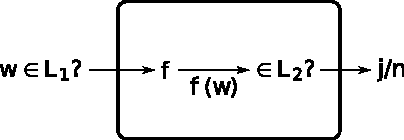
\includegraphics{kap6Reduktionsalgorithmus}
  \caption{Falls $L_1 \le_p L_2$ und $L_2 \in \mathsf{P}$ lässt sich ein Polynomialzeitalgorithmus finden, der $L_1$ entscheidet. Dazu wird die Eingabe $w$ für $L_1$ in polynomieller Zeit in eine Eingabe $f(w)$ für $L_2$ gewandelt und dann der Polynomialzeitalgorithmus von $L_2$ angewandt. Zu sehen ist ein solcher Polynomialzeitalgorithmus, der $L_1$ entscheidet.}
  \label{kap6Reduktionsalgorithmus}
\end{figure}

$f$ ist für die Umwandlung der Eingabe zuständig und hat Laufzeit $p(n)$, wobei $p$ ein Polynom sei. Der Algorithmus für $L_2$ habe Laufzeit $q(n)$. Daraus folgt $|f(w)| \le p(n)$, die gesamte Laufzeit des in Abbildung \vref{kap6Reduktionsalgorithmus} gezeigten Algorithmus ist $\le p(n) + q(p(n))$, wobei $q(p(n))$ polynomiell ist, wenn $p, q$ polynomiell sind.

\begin{Def}[\textsf{NP}-schwer]
  \hspace{\parindent}Eine Sprache $L$ heißt \textit{\textsf{NP}-schwer} (\textit{\textsf{NP}-hard}) genau dann, wenn $L' \le_p L$ für alle $L' \in \mathsf{NP.}$
\end{Def}

\begin{Def}[\textsf{NP}-vollständig]
  \hspace{\parindent}$L$ heißt \textit{\textsf{NP}-vollständig} (\textit{\textsf{NP}-complete}) genau dann, wenn $L$ \textsf{NP}-schwer und $L \in NP$.
\end{Def}

\begin{Anm}
  \hspace{\parindent}Falls es eine Sprache $L$ gibt, die \textsf{NP}-schwer ist und $L \in P$, dann $P = NP$.
\end{Anm}

\begin{Anm}\label{transitiveReduktion}
  \hspace{\parindent}Falls $L_1 \le_p L_2$ und $L_1$ ist \textsf{NP}-schwer, dann ist auch $L_2$ \textsf{NP}-schwer. Das heißt $\le_p$ ist transitiv (siehe auch Abbildung \vref{kap6ReduktionTransitiv}).
\end{Anm}

\begin{figure}[htb]
  \centering
  \includegraphics[scale=.75]{kap6ReduktionTransitiv}
  \caption{$\le_p$ ist transitiv: Falls $L_1 \le_p L_2$ und $L_1$ ist \textsf{NP}-schwer, dann ist auch $L_2$ \textsf{NP}-schwer.}
  \label{kap6ReduktionTransitiv}
\end{figure}

Gibt es überhaupt \textsf{NP}"=volltständige Probleme? Wenn einmal von einem Problem gezeigt ist, dass es \textsf{NP}"=vollständig ist können wir Polynomialzeit"=Reduktion anwenden, um es von weiteren Problemen zu zeigen.

\section{Schaltkreis"=Erfüllbarkeit}
Das Problem der \textsc{Schaltkreis"=Erfüllbarkeit} ist auch bekannt als \textsc{CSat} (\textit{circuit satisfiability}). Wir werden das Problem kurz vorstellen und dann nachweisen, dass es \textsf{NP}"=vollständig ist.

Gegeben ist einen Schaltkreis, wie wir ihn zum Beispiel in Abbildung \vref{kap6XOR} sehen.
% Gefragt ist, ob es eine \textit{erfüllende Belegung} für seine Eingänge gibt, das heißt, ob man seine Eingänge so mit $0$ und $1$ belegen kann, dass am Ausgang eine $1$ entsteht?

\begin{figure}[htb]
  \centering
  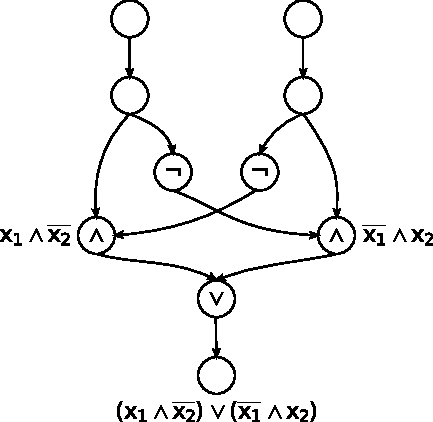
\includegraphics[scale=.66]{kap6XOR}
  \caption{Ein Schaltkreis: Aufgebaut aus AND, OR und NOT erhalten wir die boolsche Funktion $(x_1 \wedge \overline{x_2}) \vee (\overline{x_1} \wedge x_2)$ auch bekannt als \textit{XOR}.}
  \label{kap6XOR}
\end{figure}

Formal betrachtet ist eine Schaltkreis ein gerichteter azyklischer Graph, dessen Knoten wie in Abbildung \vref{kap6KnotenMarkierung} markiert sind.
\begin{figure}[htb]
  \centering
  \subfloat[Eingänge]{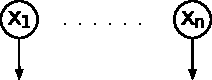
\includegraphics{kap6KnotenMarkierungEingaenge}}\\
  \subfloat[Ein Ausgang]{\makebox[.5\textwidth][c]{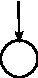
\includegraphics{kap6KnotenMarkierungAusgang}}}\\
  \subfloat[Eine allgemeine Verzweigung, eine UND-Verknüpfung, eine ODER-Verknüpfung und eine Negation]{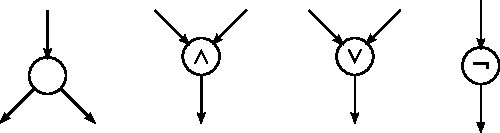
\includegraphics{kap6KnotenMarkierungVerzweigungVerknuepfungen}}
  \caption{Ein Schaltkreis ist ein gerichteter azyklischer Graph, dessen Knoten wie abgebildet markiert sind.}
  \label{kap6KnotenMarkierung}
\end{figure}

Einem Schaltkreis mit $n$ Eingängen kann in kanonischer Weise eine Boolesche Funktion $f : \{0,1\}^n \to \{0,1\}$ zugeordnet werden. Jedem der $n$ Eingänge wird dabei eine der Eingabevariablen $\alpha_i$ zugeordnet. Dann wird dem Ausgabeknoten bei Eingabe $\alpha_1 \ldots \alpha_n$ ein Bit zugeordnet, das $f(\alpha_1, \ldots, \alpha_n)$ entspricht.

\begin{Def}[erfüllbarer Schaltkreis]
  \hspace{\parindent}Ein Schaltkreis $C$ heißt \textit{erfüllbar} genau dann, wenn es eine Eingabe $\alpha_1, \ldots, \alpha_n$ gibt mit $f_c(\alpha_1, \ldots \alpha_n) = 1$.
\end{Def}

Das Problem der Schaltkreis"=Erfüllbarkeit (\textsc{CSat}) beschäftigt sich genau damit: gegeben ist ein Schaltkreis $C$. Ist $C$ erfüllbar?

$\mathsc{CSat} \in \mathsf{NP}$, denn als Zeuge $x$ dient eine Eingabe ($\alpha_1, \ldots, \alpha_n$), mit der der Verifikationsalgorithmus $A(C,x)$ nachprüft, ob $C$ bei Eingabe $x$ eine 1 liefert. Das geht leicht in polynomieller Zeit.

\begin{Satz}[Cook, 1970]
  \hspace{\parindent}\textsc{CSat} ist \textsf{NP}"=vollständig.
\end{Satz}

\begin{Bem}
  \hspace{\parindent}Cook hat ursprünglich nicht für \textsc{CSat} gezeigt, dass es \textsf{NP}"=vollständig ist, sondern für die Erfüllbarkeit boolescher Formeln (\textsc{Sat}). Die Analogie ist leicht zu sehen.
\end{Bem}

\begin{Bew}[Satz von Cook]
  \hspace{\parindent}Zunächst die Beweisidee:
  
  \begin{itemize}
    \item \textsc{CSat} ist in \textsf{NP}: siehe oben.
    \item \textsc{CSat} ist \textsf{NP}-schwer: zu zeigen ist, dass für beliebiges $L \in NP$ gilt $L \le_p \text{\textsc{CSat}}$. Das heißt wir wollen eine Funktion $f$ beschreiben, die in polynomieller Zeit berechenbar ist, mit $w \in L \Leftrightarrow f(w) \in \mathsc{CSat}$. Dabei ist $f(w)$ natürlich ein Schaltkreis.
  \end{itemize}
  
  Wir werden den Beweis nicht bis ins letzte Detail durchgehen, wollen uns aber die Konstruktion des Schaltkreises, also die oben als $f$ bezeichnete Funktion näher ansehen.
  
  Wir wissen: es existiert ein Algorithmus $A$, $k \in \mathbb{N}$ mit $w \in L \Leftrightarrow \exists x : |x| \le |w|^k$ und $A(w,x) = 1$. Sei $M_A=(Q, \Sigma, \delta, q_0)$ eine deterministische Einband"=Turingmaschine, die $A$ in polynomieller Zeit berechnet. Für Eingabe $w$ konstruieren wir einen Schaltkreis $S_w$ mit $w \in L \Leftrightarrow S_w \text{ ist erfüllbar}$. Wir bauen also einen Schaltkreis $f(w)$ der einer festen Verdrahtung der Rechnung entspricht, die $M_A$ ausführt. Der Schaltkreis hat $|w|^k$ Eingänge, und einen fest vorgegebenen Teil $w$, der neben den Eingängen als Teil der Eingabe gesehen werden kann. Die Eingänge des Schaltkreises dienen der Eingabe des Zeugen $x$.
  
  Der Schaltkreis besteht aus einzelnen Bausteinen von denen jeder einer Anwendung der Überführungsfunktion $\delta$ der Turingmaschine $M_A$ entspricht.
  \[ \delta(a,q) = (\tilde{a}, D, \tilde{q}) \]
  Das heißt: wird das Zeichen $a$ im Zustand $q$ gelesen, so geht $M_A$ in den Zustand $\tilde{q}$ über überschreibt $a$ mit $\tilde{a}$ und bewegt den Kopf in Richtung $D \in \{R, L, 0\}$. Abbildung \vref{kap6CSATBaustein} veranschaulicht einen solchen Baustein.
  
  \begin{figure}[htb]
    \centering
    \includegraphics[scale=.45]{kap6CSATBaustein}
    \caption{k ist ein Kontrollbit, a sind mehrere Eingänge, die Zeichen $a$ codieren, q mehrere Eingänge, die den Zustand $q$ codieren.}
    \label{kap6CSATBaustein}
  \end{figure}

% Vorlesung 24, 28.01.2011 (Fr)
  Um die Bausteine miteinander verknüpfen zu können, betrachten wir die Ausgabe des Bausteins genauer:
  \begin{align*}
    q' &= \begin{cases} \tilde{q} & \text{ falls } k=1 \\ 0 \ldots 0 & \text{ sonst (codiert: keinen Zustand)} \end{cases} \\
    k' &= \begin{cases}000 & \text{ falls } k=0 \\ 100 & \text{ falls } k=1, D=L \\ 010 & \text{ falls } k=1, D=0 \\ 001 & \text{ falls } k=1, D=R \end{cases} \\
    a' &= \begin{cases} \tilde{a} & \text{ falls } k=1 \\ a & \text{ sonst}\end{cases}
  \end{align*}
  
  Wie sieht nun der gesamte Schaltkreis aus? Sei $n=|w|$ und $k$ aus der Defintion von $L \in \mathsf{NP}$. Die Laufzeit der Turingmaschine $M_A$ sei $P(N)$ mit $N = |w| + |x| \le n + n^k$. Der Schaltkreis $S_w$ ist dann ein $P(N) \times P(N)$-Schema aus $B$"=Bausteinen, wie in Abbildung \vref{kap6SchaltkreisSchema}.
  
  \begin{figure}[htb]
    \centering
    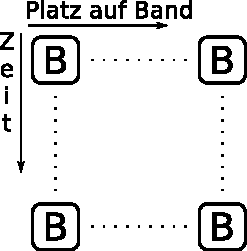
\includegraphics{kap6SchaltkreisSchema}
    \caption{Der Schaltkreis $S_w$ ist ein $P(n) \times P(N)$-Schema aus $B$-Bausteinen. Die Zeilen entsprechen den Schritten, die $M_A$ macht, daher braucht es $P(N)$ viele. Die Spalten entsprechen den Zellen, die auf dem Band von $M_A$ genutzt werden. Auch hier braucht es $P(N)$ viele, da eine Turingmaschine in jedem Schritt maximal eine Zelle durchwandert. $M_A$ kann also maximal $P(N)$ viele Zellen nutzen.}
    \label{kap6SchaltkreisSchema}
  \end{figure}
  
  Die Verknüpfung der Bausteine miteinander betrachten wir beispielhaft am Stein $B_{ij}$, der in der $i$-ten Zeile und $j$-ten Spalte des Schemas steht, also der $j$-ten Zelle des Bandes zum Zeitpunkt $i$ entspricht. Diesen Baustein und seine Umgebung sehen wir in Abbildung \vref{kap6VerknuepfungDerBausteine}. In der selben Abbildung sehen wir auch eine Schaltung, um drei Eingänge komponentenweise disjunktiv zu verknüpfen. Eine solche Schaltung nutzen wir für die Eingänge $q$ und $k$.
  
  \begin{figure}[htp]
    \centering
    \includegraphics[height=.33\textheight]{kap6VerknuepfungDerBausteine}
    \caption{Die Ausgänge $L, 0, R$ der drei Bausteine aus der bevorstehenden Reihe werden komponentenweise mittels $\vee$ verknüpft und zum Eingang $k$ des Bausteins geführt. Selbiges passiert mit den Ausgängen $q$ der drei Bausteine der bevorstehenden Reihe. die mit dem Eingang $q$ verbunden werden. Der Ausgang $a$ des zuvorstehenden Bausteins wird direkt mit dem Eingang $a$ verbunden.	}
    \label{kap6VerknuepfungDerBausteine}
  \end{figure}
  
  Der Eingang $k$ entscheidet, ob ein Baustein \textit{aktiv} geschaltet ist, oder nicht. Ein Baustein erhält immer das aktuelle Zeichen der Zelle des Bandes, die er repräsentiert. $a$ wird also immer weiter gereicht, auch wenn ein Baustein nicht aktiv ist. Wird ein Baustein aktiviert, so erhält er auch den richtigen Zustand. Zwei der Vorgängerbausteine geben $0 \ldots 0$ aus, was komponentenweise mit dem Ausgang $q$ des aktiven dritten Vorgängerbausteins disjunktiv verknüpft wird. Letzterer gibt den aktuellen Zustand an den neuen aktiven Baustein weiter. Am Ausgang $q'$ der aktiven Zelle entsteht so immer der richtige aktive Zustand.
  
  \begin{figure}[hbp]
    \centering
    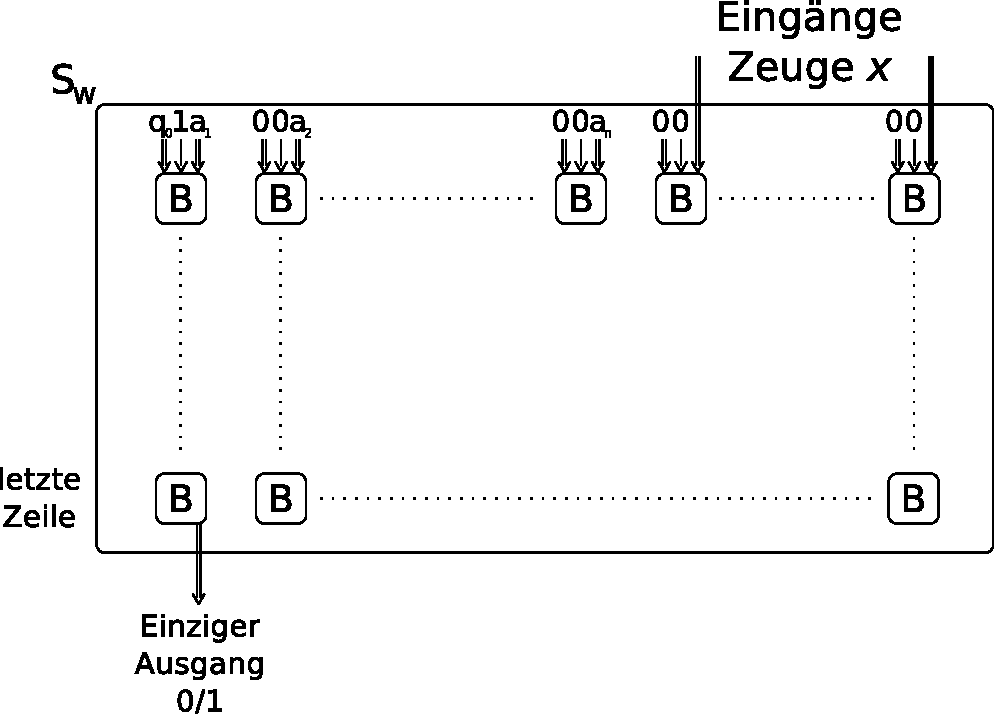
\includegraphics[width=.75\textwidth]{kap6SchaltkreisUeberblick}
    \caption{Überblick über den gesamten Schaltkreis. Sei $w= a_1 \ldots a_n$ und $q_0$ Anfangszustand von $M_A$. Der Zeuge $x$ wird über die Eingänge eingegeben, es gibt nur einen Ausgang, der genau wie der Verifikationsalgorithmus $0$ oder $1$ ausgibt (beziehungsweise das codierte Wort für $0$ oder $1$).}
    \label{kap6SchaltkreisUebersicht}
  \end{figure}
  
  In Abbildung \vref{kap6SchaltkreisUebersicht} bekommen wir einen Überblick über den gesamten Schaltkreis $S_w$. Wir nehmen an, dass $M_A$ das codierte Wort $10 \ldots 0$ auf das Band schreibt, falls das Ergebnis der Rechnung $1$ ist. Andernfalls schreibt $M_A$ $0 \ldots 0$ in die erste Zelle des Bandes. Nun wäre noch formal zu zeigen: $w \in L \Leftrightarrow S_w \text{ erfüllbar}$.
  
  \glq$\Rightarrow$\grq: Aus $w\in L$ folgt, dass es einen Zeugen $x$ gibt, für den $A(w,x)=1$. Die Codierung von $x$ ist dann eine erfüllende Belegung von $S_w$, da $S_w$ die Rechnung von $M_A$ "`simuliert"'. Das heißt aus $w \in L$ folgt $S_w$ ist erfüllbar.
  
  \glq$\Leftarrow$\grq: Angenommen $S_w$ ist erfüllbar. Dann gibt es eine erfüllende Belegung der Eingänge von $S_w$. Diese Belegung entspricht dann einem Zeugen $x$ für $w \in L$. Denn dann ist $A(w,x) =1$, da $S_w$ die Rechnung von $M_A$ "`simuliert"'. Das heißt aus $S_w$ ist erfüllbar folgt $w \in L$.
  
  Für einen vollständigen Beweis fehlen noch viele Kleinigkeiten. Die Beweisidee, speziell der Aufbau des Schaltkreises sollte aber klar geworden sein.  Damit wären alle Probleme in \textsf{NP} auf \textsc{CSat} reduzierbar.
  
  Die Konstruktion von $S_w$ aus $w$ ist in polynomieller Zeit möglich: das Schema hat $P(N) \cdot P(N)$ $B$"=Bausteine. Ein $B$"=Baustein hat konstante Größe, unabhängig von $w$ oder $x$. Die Konstruktion des gesamten Schaltkreises ist daher in $\mathcal{O}(P(N) \cdot P(N)) = \mathcal{O}(P(n+n^k)^2)$ möglich. $P(n+n^k)^2$ ist ein Polynom in $n$.
\end{Bew}

\begin{Anm}
  \hspace{\parindent}So ein Schaltkreis lässt sich immer Bauen, da $\wedge$, $\vee$, $\neg$ eine vollständige Basis für Booleschen Funktionen bilden.
\end{Anm}

\section{Weitere NP"=vollständige Probleme}
Der Beweis, dass \textsc{CSat} \textsf{NP}-vollständig ist, ist recht umfangreich. Da polynomielle Reduktion transitiv ist, können wir für weitere Probleme leichter zeigen, dass sie \textsf{NP}-schwer sind, in dem wir \textsc{CSat} auf diese Probleme reduzieren. Können wir auch noch nachweisen, dass sie in \textsf{NP} liegen, so haben wir nachgewiesen, dass auch sie \textsf{NP}"=vollständig sind.

\subsection{SAT (satisfiability)}
Gegeben sind Variablen $x_1, x_2, \ldots$ und Operationen (einstellige Negation, zweistellige Konjunktion und zweistellig Disjunktion), zum Beispiel $(x_1 \vee x_2 \vee \overline{x}_3)\wedge(x_2 \vee x_3 \vee x_4) \wedge (\overline{x}_1 \vee x_2 \vee \overline{x}_4)$. $(\overline{x}_1 \vee x_2 \vee \overline{x}_4)$ heißt \textit{Klausel} (\textit{clause}). Negierte oder nichtnegierte Variablen, wie zum Beispiel $\overline{x_1}, x_2, \overline{x}_4$, heißen \textit{Literale}.

\begin{Def}[Konjunktive Normalform (KNF)]
  \hspace{\parindent}Eine aussagenlogische Formel ist in \textit{konjunktive Normalform} (KNF), wenn sie nur aus Konjunktionen von disjunktiv verknüpften Literalen besteht. Das zuvor angegebene Beispiel, ist in KNF angegeben.
\end{Def}

\begin{Anm}
  \hspace{\parindent}Aus dem Grundstudium wissen wir, dass alle aussagenlogische Formeln in KNF überführt werden können.
\end{Anm}

\begin{Def}[Erfüllbarkeit boolescher Formeln]
  \hspace{\parindent}Eine Formel heißt \textit{erfüllbar} genau dann, wenn die Variablen der Formel so mit Wahrheitswerten (0,1) belegt werden können, dass der Wert der Formel insgesamt $1$ wird.
\end{Def}

Die oben beispielhaft angegebene Formel ist erfüllbar, denn $x_1 \leftarrow 1, x_2 \leftarrow 1, x_3 \leftarrow 1, x_4 \leftarrow 0$ ist eine \textit{erfüllende Belegung}.

Das Problem \textsc{Sat} (\textit{satisfiability}) befasst sich mit der Erfüllbarkeit aussagenlogischer (boolescher) Formeln. Gegeben ist eine aussagenlogische Formel $q$ (in KNF). \textsc{Sat} fragt ob $q$ erfüllbar ist oder nicht.

\begin{Anm}
  \hspace{\parindent}Jede boolesche Formel kann wie gesagt in KNF gebracht werden. Im schlimmsten Fall hat die Formel in KNF jedoch exponentielle Länge im Vergleich zur ursprünglichen Formel. Geht es nicht um strenge Äquivalenz, sondern um Erfüllbarkeitsäquivalenz, lässt sich zu jeder booleschen Formel durch einfügen neuer Variablen eine KNF finden, deren Länge linear im Vergleich zur Länge der ursprünglichen Formel liegt. \textsc{Sat} betrachtet ausschließlich die Erfüllbarkeit einer aussagenlogischen Formel. Ohne Beschränkung der Allgemeinheit können wir daher davon ausgehen, dass diese in KNF vorliegt.
\end{Anm}

\begin{Satz}
  \hspace{\parindent}\textsc{Sat} ist \textsf{NP}"=vollständig.
\end{Satz}

\begin{Bew}
  \hspace{\parindent}$\mathsc{Sat} \in \mathsf{NP}$, denn zu jeder erfüllbaren Formel $\varphi$ dient uns als Zeuge eine erfüllende Belegung. Ein Verifikationsalgorithmus evaluiert $\varphi$ mit einer solchen Belegung. Um zu zeigen, dass \textsc{Sat} \textsf{NP}"=vollständig ist, müssen wir aber noch zeigen, dass \textsc{Sat} \textsf{NP}-schwer ist. Das zeigen wir durch eine Reduktion $\mathsc{CSat} \le_p \mathsc{Sat}$.
  
  Gegeben sei ein Schaltkreis $S$. Wir konstruieren eine Formel $\varphi_s$, so dass $S$ erfüllbar ist genau dann, wenn $\varphi_s$ erfüllbar ist, wie folgt.
  $\varphi_s$ hat die Variablen $x_1, \ldots, x_n$ für die Eingänge des Schaltkreises und $y_1, \ldots, y_k$ für die $\neg, \wedge, \vee$ Gatter des Schaltkreises. Es werden nun Klauseln, wie in Abbildung \vref{kap6SatRedCSat} dargestellt, gebildet.
  
  \begin{figure}[htb]
    \centering
    \subfloat[Eine solche Schaltung wird in eine Klausel $y_m \equiv y_k \vee y_l$ umgewandelt, wobei $a \equiv b$ Abkürzung für $(a \vee \overline{b}) \wedge (\overline{a} \vee b)$ ist. Eine konjunktive Schaltung ($\wedge$-Gatter) wird dem entsprechend umgesetzt.\label{kap6SatRedCSat1}]{\makebox[15em][c]{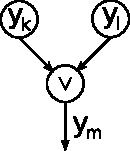
\includegraphics{kap6SatRedCSat1}}}\hspace{1em}
    \subfloat[Ein Gatter zur Negation wird durch folgende einfache Klausel umgesetzt: $\overline{y}_k \equiv y_m$.\label{kap6SatRedCSat2}]{\makebox[15em][c]{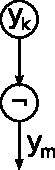
\includegraphics{kap6SatRedCSat2}}}
    \caption{Reduktion von \textsc{CSat} auf \textsc{Sat}: Bildung von Klauseln. $y_k$ und $y_l$ können Eingänge oder andere Gatter sein.}
    \label{kap6SatRedCSat}
  \end{figure}
  
  Die Klauseln werden nun für alle Gatter des Schaltkreises gebildet. Die Formel $\varphi_s$ entspricht nun der Konjuktion all dieser $(y_m \equiv y_k \vee y_l)$, $(y_m \equiv y_k \wedge y_l)$, $(y_m \equiv \overline{y}_k)$ Teilformeln.

  Zu zeigen ist: $S$ ist erfüllbar genau dann, wenn $\varphi_s$ erfüllbar ist. Wir wollen dazu die Beweisidee vorstellen und nicht den vollständigen eigentlichen Beweis.
  
  \glq$\Rightarrow$\grq: Sei $\alpha_1 \ldots \alpha_n$ eine erfüllende Eingabe. Belege die Variablen $x_i \leftarrow \alpha_i \quad i=1, \ldots, n$ und $y_1, \ldots, y_k$ mit den Werten, die die entsprechenden Gatter im Schaltkreis produzieren, bei Eingabe der erfüllenden Belegung $\alpha_1 \ldots \alpha_n$ für $\varphi_s$. Per Induktion lässt sich beweisen, dass aus $S$ ist erfüllbar folgt, dass auch $\varphi_s$ erfüllbar ist. Die Formel $\varphi_s$ wurde genauso angelegt, dass dieser Schluss folgt.
   %Müsste man jetzt eigentlich noch per Induktion über ... zeigen, der Schaltkreis wurde allerdings genauso angelegt, dass das stimmt.
  
  \glq$\Leftarrow$\grq: Betrachte erfüllende Belegung für $\varphi_s$.
  \[ \begin{array}{rcl} x_1 & \leftarrow & \alpha_1 \\ & \vdots & \\x_n & \leftarrow & \alpha_n \\ y_1 & \leftarrow & \vdots\\ & \vdots & \\ y_k & \leftarrow & \vdots \end{array}\]
  Gib $\alpha_1 \ldots \alpha_n$ als Eingabe an $S$. Aus der Konstruktion von $\varphi_s$ folgt, dass $S$ dann erfüllt wird. Gibt es also eine erfüllende Belegung für $\varphi_s$, so ist auch $S$ erfüllbar.
\end{Bew}

% vorlesung 25, 31.01.2011 (Mo)
\subsection{3SAT}
\textsc{3Sat} ist eine spezielle Form des Problems \textsc{Sat}. \textsc{Sat} formuliert die Frage, ob eine aussagenlogische Formel $\varphi$ erfüllbar ist. \textsc{Sat} erwartet, dass $\varphi$ in KNF vorliegt. \textsc{3Sat} untersucht die selbe Frage, stellt jedoch noch die Bedingung auf, dass jede Klausel von $\varphi$ aus maximal 3 Literalen besteht. \textsc{3Sat} ist für sich genommen eigentlich nicht sehr interessant, auch wenn trotz der Beschränkung gezeigt werden kann, dass es \textsf{NP}-vollständig ist. Es ist jedoch technisch hilfreich, wenn durch Reduktion gezeigt werden soll, dass andere Probleme \textsf{NP}"=vollständig sind.

\begin{Beh}
  \hspace{\parindent}\textsc{3Sat} ist \textsf{NP}"=vollständig.
\end{Beh}

\begin{Bew}
  \hspace{\parindent}Den Beweis, dass \textsc{3Sat} \textsf{NP}-schwer ist, führen wir durch eine Reduktion von \textsc{Sat} auf \textsc{3Sat}: $\mathsc{Sat} \le_p \mathsc{3Sat}$.
  
  Sei $\varphi=C_1 \wedge \ldots \wedge C_k$ eine Instanz für \textsc{Sat}, wobei $C_i$ Klauseln sind. Zu jeder Klausel $C=(y_1 \vee \ldots \vee y_n)$, die aus den Literalen $y_i$ ($i=1, \ldots, n$) besteht, konstruieren wir eine Formel $C'$ in 3KNF (KNF mit $\le 3$ Literalen pro Klausel) wie folgt, wenn $n > 3$:
  \[ (y_1 \vee y_2 \vee z_1) \wedge (\overline{z}_1 \vee y_3 \vee z_2) \wedge \ldots \wedge (\overline{z}_{n-3} \vee y_{n-1} \vee z_{n-2}) \wedge (\overline{z}_{n-2} \vee y_n) \]
  Dabei sind $z_i$ neue zusätzliche Variablen. Diese Konstruktion führen wir nun für alle Klauseln von $\varphi$ aus und verbinden die entstehenden $C'$ konjunktiv. Wir erhalten eine Formel $\varphi'$ in 3KNF.
  
  Dann gilt: eine erfüllende Belegung von $C$ für $y_1 \ldots y_n$ kann zu einer erfüllenden Belegung von $C'$ für $y_1, \ldots, y_n, z_1, \ldots, z_{n-2}$ erweitert werden. Eine erfüllende Belegung von $C$ muss mindestens ein $y_i$ auf $1$ setzen. Die entsprechende Klausel in $C'$ sieht aus wie folgt: $\overline{z}_{i-2} \vee y_i \vee z_{i-1}$. Wir belegen $z_1, \ldots, z_{i-2}$ mit $1$ und $z_{i-1}, \ldots, z_{n-2}$ mit $0$. $C'$ ist dann erfüllt, denn $z_1$ bis $z_{i-2}$ sind erfüllt, $y_i$ ist erfüllt und $\overline{z}_{i-1}$ bis $\overline{z}_{n-2}$ sind auch erfüllt. Es folgt: ist $\varphi$ erfüllbar, so ist auch $\varphi'$ erfüllbar (eine erfüllende Belegung von $\varphi$ kann ja wie geschildert zu einer erfüllenden Belegung von $\varphi'$ erweitert werden).
  
  Wenn $\varphi'$ erfüllbar ist, ist auch $\varphi$ erfüllbar. Denn es muss eine erfüllende Belegung von $\varphi'$ geben und diese Belegung muss in jeder Klausel $C'$ mindestens ein $y_i$ auf $1$ setzen. Angenommen das ist nicht so und es gibt eine erfüllende Belegung für eine Klausel $C'$ bei der alle $y_i$ auf $0$ gesetzt sind. Dann muss $z_1 = 1$ gesetzt sein, damit die erste Klausel erfüllt ist. Selbiges gilt für $z_2$ und die zweite Klausel und so weiter. Damit alle Klauseln bis einschließlich der vorletzten Klausel erfüllt sind müssen also $z_1, z_2, \ldots, z_{n-2}$ auf $1$ gesetzt sein. Die letzte Klausel ist dann $(\overline{z}_{n-2} \vee y_n)$. Da wir $z_{n-2}$ bereits auf $1$ und $y_n$ auf $0$ gesetzt hatten ist diese Klausel dann aber nicht erfüllt, was im Widerspruch dazu steht, dass wir eine erfüllende Belegung gefunden haben, bei der alle $y_i$ auf $0$ gesetzt sind. Daher gilt: ist $\varphi'$ erfüllbar, so ist auch $\varphi$ erfüllbar.
\end{Bew}

\subsection{Probleme der Zulässigkeit Linearer Programme}
Betrachten wir kurz zwei Probleme, die sich mit der Zulässigkeit linearer Programme befassen: \textsc{0-1-LP} und \textsc{ILP}.

\textsc{0-1-LP} steht für 01 Lineare Programmierung. Gegeben sind Nebenbedingungen $Ax \le b, A \in \mathbb{Z}^{m \times n}, b \in \mathbb{Z}^m$. Gefragt ist, ob eine zulässige Lösung $x \in \{ 0,1 \}^n$ existiert. Das Problem linearer Programmierung mit einer Zielfunktion lässt sich auf dieses Problem, bei dem $c$ dem Nullvektor entspricht, leicht reduzieren.

Ganzzahlige lineare Programmierung (integer linear programming, \textsc{ILP}) hat die selben Anforderungen, fragt jedoch, ob eine zulässige Lösung $x \in \mathbb{Z}^n$ existiert, also eine ganzzahlige Lösung.

\begin{Satz}
  \hspace{\parindent}\textsc{0-1-LP} und \textsc{ILP} sind \textsf{NP}-vollständig.
\end{Satz}

Das bedeutet insbesondere, dass ganzzahlige lineare Programmierung \textsf{NP}-schwer ist. Ganzzahlige lineare Optimierung ist deutlich schwerer zu lösen als lineare Optimierung allgemein, für die es Logarithmen gibt, die immer in polynomieller Zeit arbeiten (siehe dazu Kapitel \ref{chap:LP} zur linearen Programmierung).

\begin{Bew}
  \hspace{\parindent}Den Beweis führen wir über zwei Reduktionen: $\mathsc{Sat} \le_p \operatorname{\mathsc{0-1-LP}} \le_p \mathsc{ILP}$.
  
  Zunächst wollen wir \textsc{Sat} auf \textsc{0-1-LP} reduzieren. Sei $\varphi=C_1 \wedge \ldots \wedge C_k$ eine Instanz für \textsc{Sat}, o.B.d.A. in KNF, bestehend aus den Klauseln $C_1, \ldots, C_k$. $\varphi$ ist erfüllbar, wenn es eine Belegung für $\varphi$ gibt, so dass jede Klausel \textit{wahr} wird. Wir konstruieren eine arithmetische Formel $\varphi'$, in dem wir die booleschen Operationen von $\varphi$ wie folgt umsetzen:
  \begin{itemize}
    \item die Negation $\overline{x}_i$ setzen wir um zu $(1-x_i)$,
    \item die Disjunktion $x_i \vee x_j$ setzen wir um als Addition $x_i + x_j$ und
    \item die Konjunktion kommt in einer Klausel einer Formel in KNF nicht vor.
    %\item die Konjunktion $x_i \wedge x_j$ setzen wir um als Multiplikation $x_i \cdot x_j$ und
  \end{itemize}
  Den Wert $0$ interpretieren wir als das boolesche \textit{falsch}, den Wert $1$ als das boolesche \textit{wahr}. $\varphi$ liegt o.B.d.A. in KNF vor. Jede Klausel $C_i$ werden wir nach diesen Regeln in eine Nebenbedingung umsetzen, die $\ge 1$ sein muss.
  
  Betrachten wir zum Beispiel folgende aussagenlogische Formel:
  \[ \varphi = (x_1 \vee x_2 \vee x_3) \wedge (x_1 \vee \overline{x}_2) \wedge (x_2 \vee \overline{x}_3) \wedge (\overline{x_1} \vee \overline{x_2} \vee \overline{x}_3) \]
  Wir erhalten dann folgende Nebenbedingungen:
  \begin{align*}
    x_1 + x_2 + x_3 & \ge 1\\
    x_1 + (1 - x_2) & \ge 1\\
    x_2 + (1 - x_3) & \ge 1\\
    (1 - x_1) + (1 - x_2) + (1 - x_3) & \ge 1
  \end{align*}
  Wir multiplizieren alle Nebenbedingungen mit $-1$ und bringen die Einsen aus den negierten Variablen ($1 - x_i$) auf die rechte Seite der Ungleichungen, um sie in die gewünschte Form $Ax \le b$ zu bringen und erhalten:
  \begin{align*}
      - x_1 - x_2 - x_3 & \le -1\\
      - x_1 + x_2 & \le 0\\
      - x_2 + x_3 & \le 0\\
      x_1 + x_2 + x_3 & \le 2
  \end{align*}
  
  Gibt es eine zulässige Lösung $x \in \{ 0, 1 \}^n$, so ist $\varphi$ erfüllbar. Denn eine entsprechende Lösung gibt für jede Variable $x_i$ eine Belegung mit $0$ oder $1$ vor. In jeder Nebenbedingung wird dadurch mindestens eine nichtnegierte Variable auf $1$ gesetzt oder mindestens eine negierte Variable auf $0$. Nichtnegierte Variablen die auf $1$ gesetzt werden sorgen dafür, dass die Klause wahr wird und die Nebenbedingung einen Wert von mindestens $1$ annimmt. Negierte Variablen, die auf $0$ gesetzt sind sorgen dafür, dass die Negation in der Klause erfüllt wird und die Nebenbedingung erfüllt wird, denn $1-0 \ge 1$ gilt als erfüllt. \textsc{0-1-LP} ist nur erfüllt, wenn alle Nebenbedingungen erfüllt sind. $\varphi$ ist nur erfüllt, wenn alle Klauseln erfüllt sind.
  
  Ist $\varphi$ erfüllbar, so ist es auch das oben konstruierte lineare Programm. Die Belegung erfüllt jede Klausel von $\varphi$. Das heißt jede Klausel muss mindestens eine nichtnegierte Variable enthalten, die auf $1$ gesetzt wird oder mindestens eine negierte Variable, die auf $0$ gesetzt wird. Entsprechend lässt sich eine zulässige Lösung für das obige \textsc{0-1-LP} konstruieren, denn die Nebenbedingungen sind aus diesen Klauseln hergeleitet. Die enthaltene nichtnegierte Variable, die auf $1$ gesetzt ist oder die enthaltene negierte Variable, die auf $0$ gesetzt ist, erfüllt die entsprechende Nebenbedingung.
  
  Die Reduktion $\operatorname{\mathsc{0-1-LP}} \le_p \mathsc{ILP}$ ist Teil der Übung.
  % http://www.scribd.com/doc/184860/Integer-Programming
\end{Bew}


\subsection{Clique}
Gegeben ist ein Graph $G=(V,E)$ und eine Zahl $k \in \mathbb{N}$. Enthält $G$ eine \textit{Clique} der Größe $k$? Eine \textit{Clique} ist ein vollständiger Teilgraph, also eine Teilmenge $V' \subset V$, so dass $\{x, y\} \in E$ für alle $x, y \in V', x \neq y$ erfüllt ist.

\begin{Satz}
  \hspace{\parindent}\textsc{Clique} ist \textsf{NP}-vollständig.
\end{Satz}

\begin{Bew}
  \hspace{\parindent}$\mathsc{Clique} \in \mathsf{NP}$, denn als Zeuge dient uns eine Teilmenge $V' \subset V$ der Größe $k$ (falls $k \le n$). Der Verifikationsalgorithmus prüft, ob je zwei Knoten in $V'$ verbunden sind.
  
  Um zu zeigen, dass \textsc{Clique} \textsf{NP}-schwer ist, zeigen wir $\mathsc{3SAT} \le_p \mathsc{Clique}$. Sei $\varphi$ eine Eingabe für \textsc{3Sat}. Wir müssen dann einen Graph $G_{\varphi}$ konstruieren und eine Zahl $k \in \mathbb{N}$ finden, so dass $G_{\varphi}$ eine Clique der Größe $k$ enthält, genau dann, wenn $\varphi$ erfüllbar ist.
  
  Die Eingabe für \textsc{3Sat} ist eine aussagenlogische Formel $\varphi = C_1 \wedge \ldots \wedge C_k$, die aus Klauseln $C_i = y_{i1} \vee y_{i2} \vee y_{i3}$ mit den Literalen $y_{ij}$ besteht. $G_{\varphi}$ enthält als Knoten alle Literale aller Klauseln. Wir fügen eine Kante zwischen $y_{ij}$ und $y_{lm}$ genau dann ein, wenn $i \neq l$ und $y_{ij} \neq \overline{y}_{lm}$. Die Größe der Clique $k$ setzen wir auf die Anzahl der Klauseln. Abbildung \vref{kap6Red3SatClique} demonstriert das an einem Beispiel.
  
  \begin{figure}[htb]
    \centering
    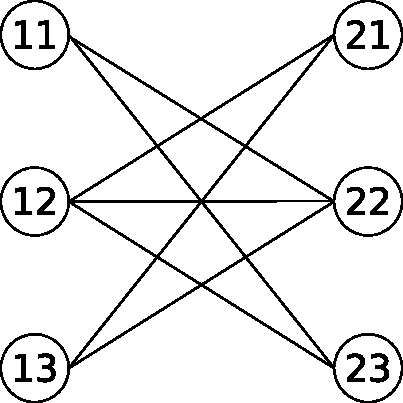
\includegraphics[scale=.6]{kap6Red3SatClique}
    \caption{Zur Formel $\varphi =(x_1 \vee \overline{x}_2 \vee x_3) \wedge (\overline{x}_1 \vee \overline{x}_2 \vee \overline{x}_{3})$ würde der abgebildete Graph $G_{\varphi}$ konstruiert werden. Dabei wird für jedes Literal ein Knoten erzeugt. Der Knoten $11$ steht für das Literal $x_1$ aus der ersten Klausel, der Knoten $12$ für das Literal $\overline{x}_2$ aus der ersten Klausel, der Knoten $21$ für das Literal $\overline{x}_1$ der zweiten Klausel und so weiter.}
    \label{kap6Red3SatClique}
  \end{figure}
  
  Dann gilt: $G_{\varphi}$ hat eine Clique der Größe $k$ genau dann, wenn $\varphi$ erfüllbar ist.
  
  \glq$\Leftarrow$\grq: Sei $\varphi$ erfüllbar. Jede erfüllende Belegung von $\varphi$ sorgt dafür, dass in jeder Klausel mindestens ein Literal erfüllt ist. Wir wählen nun pro Klausel ein erfülltes Literal aus, beziehungsweise die Knoten, die diese Literale repräsentieren. Wir hatten zwischen zwei Knoten eine Kante gezogen, wenn die Knoten Literale repräsentieren, die weder zur selben Klausel gehören noch die negierte und nichtnegierte Variante der selben Variable sind. Da wir aus jeder Klausel ein Literal wählen und alle gewählten Literale erfüllt sind, erhalten wir eine Clique der Größe $k$, die der Anzahl der Klauseln entspricht.
  
  \glq$\Rightarrow$\grq: $G_{\varphi}$ habe eine Clique der Größe $k$. Die Literale, die diesen Knoten entsprechen, ergeben eine erfüllende Belegung für $\varphi$. Denn in der Konstruktion des Graphen hatten wir nur Kanten zwischen Knoten gezogen, deren repräsentierte Literale zu unterschiedlichen Klauseln gehören und sich nicht widersprechen. Da $k$ der Anzahl der Klauseln entspricht, haben wir in jeder Klausel mindestens ein Literal erfüllt, was dafür sorgt, dass $\varphi$ erfüllt ist.
\end{Bew}

\subsection{Überdeckende Knotenmenge (vertex cover, VC)}
Gegeben ist ein Graph $G=(V,E)$ und eine Zahl $k \in \mathbb{N}$. Existiert ein \textsc{VC} der Größe $k$? Das heißt existiert eine Teilmenge $V' \subset V$ mit $|V'|=k$, so dass jede Kante in $E$ zu mindestens einem Knoten von $V'$ inzident ist?

\begin{figure}[htb]
  \centering
  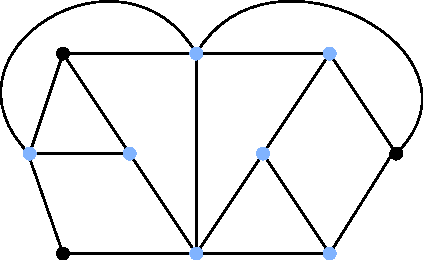
\includegraphics[scale=.75]{kap6BspVC}
  \caption{Die hellblauen Knoten des Graphen bilden ein vertex cover der Größe $7$ in ihm.}
  \label{kap6BspVC}
\end{figure}

\begin{Satz}
  \hspace{\parindent}\textsc{VC} ist \textsf{NP}"=vollständig.
\end{Satz}

\begin{Bew}
  \hspace{\parindent}$\mathsc{VC} \in \mathsf{NP}$ zu zeigen ist leicht. Ein Zeuge ist eine Knotenmenge. Ein Verifikationsalgorithmus kann zum Beispiel alle Kanten markieren, die zu den in der Knotenmenge enthaltenen Knoten inzident sind. Sind alle Kanten markiert akzeptiert er, sonst verwirft er.
  
  Das \textsc{VC} \textsf{NP}-schwer ist, zeigen wird durch die Reduktion $\mathsc{Clique} \le_p \mathsc{VC}$.
  
  Sei $G=(V, E),~k$ eine Instanz für \textsc{Clique}. Wir konstruieren den komplementären Graphen $\overline{G} = (V, \binom{V}{2} \setminus E)$, der also alle ungeordneten Paare von $V$ enthält, die nicht in $E$ enthalten sind. Sei $\overline{k}= n - k$. Dann gilt $G$ hat eine Clique der Größe $k$ genau dann, wenn $\overline{G}$ ein \textsc{VC} der Größe $\overline{k}$ hat.
  
  Angenommen $V' \subseteq V$ sei eine Clique von $G$ der Größe $k$. Dann ist $V \setminus V'$ ein VC in $\overline{G}$. Für alle Kanten $(u, v) \in \overline{G}$ gilt $(u, v) \notin E$. Daraus folgt, dass mindestens einer der Knoten $u, v$ nicht Teil von $V'$ ist, denn alle Knoten, die zu $V'$ gehören, sind paarweise durch eine Kante in $E$ verbunden (sonst wäre $V'$ keine Clique). Das bedeutet aber auch, dass mindestens einer der beiden Knoten Teil von $V \setminus V'$ sein muss. Jede Kante $(u, v) \in \overline{G}$ ist also von der Knotenmenge $V \setminus V'$ überdeckt. Die Menge $V \setminus V'$ bildet also ein VC der Größe $|V| - k$ in $\overline{G}$.
  
  Angenommen $V' \subseteq V$ ist ein VC in $\overline{G}$ und $|V'| = \overline{k}$. Für jede Kante $(u, v) \in \overline{G}$ gilt, dass $u \in V'$ oder $v \in V'$ oder $u,v \in V'$. Daraus folgt, dass für alle $w, x \notin V'$ folgt, dass $(w, x) \notin \overline{G}$. Dann muss $(w, x)$ aber in $E$ enthalten sein. Das heißt $V \setminus V'$ ist eine Clique der Größe $|V| - |V'|$, was wiederum $k$ entspricht.
\end{Bew}

%vorlesung 26, 04.02.2011 (Fr). Jens Schmidt
\subsection{Subset-Sum}
\textsc{Subset-Sum} haben wir bereits zu Beginn des Kapitels vorgestellt. Gegeben sind einige Zahlen $a_1, \ldots, a_n, b$. Existiert eine Teilmenge $I \subset \{1, \ldots, n\}$, so dass $\sum_{i \in I} a_i = b$? Es ist auch bekannt als \textsf{0-1-Rucksack} (\textsf{0-1-Knapsack}).

Wir zeigen per Reduktion, dass \textsc{Subset-Sum} \textsf{NP}-schwer ist. Dazu reduzieren wir \textsc{VC} auf \textsc{Subset-Sum}. Gesucht ist also eine Funktion $f$, so dass $w \in \mathsc{VC} \Leftrightarrow f(w) \in \operatorname{\mathsc{Subset-Sum}}$. $w$ ist ein Graph und eine Zahl $k$, $f(w)$ eine Menge von Zahlen. Wir gehen dazu wie folgt vor:
\begin{itemize}
  \item Wir bilden die Inzidenzmatrix über den Graphen $G$ des Problems \textsc{VC}.
  \item An die Inzidenzmatrix hängen wir eine $|E| \times |E|$ Einheitsmatrix an.
  \item Wir fügen links eine neue Spalte hinzu, in die ersten $|V|$ Zeilen tragen wir jeweils $1$ ein, in die folgenden $|E|$ Zeilen $0$.
  \item Wir fügen eine letzte Zeile unten an, in deren ersten Spalte wir $k$ schreiben und deren andere Spalten $2$ enthalten.
  \item Jede Zeile, bis auf die letzte, interpretieren wir nun als Viernäre Zahl. Das bildet die Menge $\{a_1, \ldots, a_n\}$ unser Eingabe für \textsc{Subset-Sum}.
  \item $b$ setzen wir wie folgt: $b = \sum_{i=0}^{|E|-1}2 \cdot 4^i + k\cdot 4^{|E|}$, das entspricht der letzten Zeile, interpretiert als viernäre Zahl.
\end{itemize}

\begin{Bsp}
  \hspace{\parindent}Betrachten wir das ganze an einem Beispiel. Als Eingabe für \textsc{VC} dient uns der Graph, der in Abbildung \vref{kap6BspRedVCSubsetSum} zu sehen ist.

  \begin{figure}[hbt]
    \centering
    \includegraphics[scale=.75]{kap6BspRedVCSubsetSum}
    \caption{Ein Graph, der uns als beispielhafte Eingabe für \textsc{VC} dient.}
    \label{kap6BspRedVCSubsetSum}
  \end{figure}
  
  Wir bilden jetzt die Inzidenzmatrix, hängen eine Einheitsmatrix der Dimension $|E|=6$ an, fügen links die Spalte und unten die letzte Zeile an. Das Ergebnis sieht aus wie folgt:
  
  \begin{center}
    \begin{tabular}{>{$}l<{$}>{$}l<{$}||>{$}c<{$}>{$}c<{$}>{$}c<{$}>{$}c<{$}>{$}c<{$}>{$}c<{$}>{$}c<{$}}
            & & & e_1 & e_2 &e_3 & e_4 & e_5 & e_6\\\hline\hline
      a_1 & v_1 & 1 & 1 & 0 & 0 & 0 & 0 & 0\\
      a_2 & v_2 & 1 & 1 & 1 & 0 & 1 & 1 & 0\\
      a_3 & v_3 & 1 & 0 & 1 & 1 & 0 & 0 & 0 \\
      a_4 & v_4 & 1 & 0 & 0 & 0 & 0 & 1 & 1 \\
      a_5 & v_5 & 1 & 0 & 0 & 1 & 1 & 0 & 1 \\\hline
      a_6    &  & 0 & 1 & & & \multicolumn{3}{c}{\multirow{3}{*}{\Huge $0$}}\\
      a_7    &  & 0 & & 1 \\
      a_8    &  & 0 & & & 1\\
      a_9    &  & 0 & \multicolumn{3}{c}{\multirow{3}{*}{\Huge $0$}} & 1\\
      a_{10} &  & 0 & & & & & 1\\
      a_{11} &  & 0 & & & & & & 1\\\hline\hline
      b      &  & k & 2 & 2 & 2 &2 & 2 & 2
    \end{tabular}
  \end{center}
  
  Die Zahl $a_5$ in diesem Beispiel berechnet sich wie folgt: $a_5 = 1 \cdot 4^0 + 1 \cdot 4^2 + 1 \cdot 4^3 + 1 \cdot 4^6$. Die Summe jeder Spalte ist übrigens $3$ (die letzte Zeile ausgelassen). Die Formel für $b$ hatten wir oben bereits angegeben: $b=\sum_{i=0}^{|E|-1}2 \cdot 4^i + k\cdot 4^{|E|}$, hier im Beispiel also $b=\sum_{i=0}^{5} 2 \cdot 4^i + k \cdot 4^6$.
\end{Bsp}

Nachdem klar ist, wie wir die Reduktion durchführen, bleibt noch zu zeigen, dass $w \in \mathsc{VC}$ gilt genau dann, wenn $f(w) \in \operatorname{\mathsc{Subset-Sum}}$.

\glq$\Rightarrow$\grq: Es existiere eine überdeckende Knotenmenge der Größe $k$ ($v_{i_1}, \ldots, v_{i_k}$). Aus der Menge $\{a_1, \ldots, a_{n+m} \}$ wählen wir jetzt $a_{i_1}, \ldots , a_{i_k}$ aus. Jede Spalte summiert sich über die ausgewählten Zeilen zu $1$ (nur einer der beiden inzidenten Knoten ist in $V'$ enthalten), oder zu $2$ (beide inzidente Knoten sind enthalten) auf. Bei den Kanten, bei denen nur einer der inzidenten Knoten in $V'$ enthalten ist (Spaltensumme beträgt $1$) wählen wir zusätzlich noch die entsprechende Zeile aus der Einheitsmatrix aus (in unserem Beispiel sind das $a_6$ bis $a_{11}$). Die Summe über die erste Spalte wird so immer $k$ groß, die Summe über die anderen Spalten $2$ und somit folgt $f(w) \in \operatorname{\mathsc{Subset-Sum}}$ aus $w \in \mathsc{VC}$.

\glq$\Leftarrow$\grq: Es existiere eine Menge von Zeilen, die aufsummiert $b$ ergeben. Wegen $k$ an erster Stelle von $b$, muss diese Menge genau $k$ Zeilen der Inzidenz"=Matrix enthalten. Das repräsentiert einen Vertex"=Cover"=Kandidaten. Jede Spalte summiert sich zu $2$ auf, woraus folgt, dass mindestens ein Knoten je zugehöriger Kante enthalten ist, alle Kanten sind also überdeckt. Aus $f(w) \in \operatorname{\mathsc{Subset-Sum}}$ folgt also $w \in \mathsc{VC}$.

Zu Laufzeit und Platzbedarf sei kurz angemerkt, dass eine Inzidenzmatrix aus vielen Nullen und Einsen besteht. Alle oben verwendete Zahlen sind kleine Zahlen, alles nur je ein Bit. Der Platzbedarf (man denke an das logarithmische Kostenmaß) geht also in der $\Theta$"=Notation unter. Sei $n = |V|$ und $k$ eine beliebige Zahl aus $\mathbb{N}$. $f$ ist in polynomieller Zeit berechenbar. Die Eingabelänge liegt in $\Theta (n^2 + \log k)$, die Laufzeit in $\Theta (|V| \cdot |E| + |E|^2 + \log k)$. Jede 4-näre Zahl kann auch binär dargestellt werden, codiert durch 2 Bits. Das heißt für jede viernäre Zahl kommt einfach noch Faktor 2 dazu, was wieder in $\Theta$ untergeht. Wir wissen $|E| \le |V|^2$. Deshalb liegt die Laufzeit in $\Theta (n^4 + \log k)$, was quadratische in Bezug auf die Eingabelänge ist.

\subsection{Hamiltonkreis (hamiltonian circuit)}

\begin{Def}[Hamiltonkreis (hamiltonian circuit)]
  \hspace{\parindent}In einem Graphen heißt ein Kreis $w$ \textit{Hamiltonkreis} (\textit{hamiltonian circuit}), wenn er jeden Knoten genau einmal enthält. Man unterscheidet zwischen einem Hamiltonkreis in einem gerichtetem und einem Hamiltonkreis in einem ungerichteten Graphen.
\end{Def}

Das bekannte \textit{Problem des Handlungsreisenden} (\textit{travelling salesman problem}, \textsc{TSP}) ist ein Spezialfall, bei dem in einem gerichteten und gewichtetem Graphen nach einem Hamiltonkreis mit minimalen Kosten gefragt wird.

Die Frage, ob es in einem ungerichteten Graphen einen Hamiltonkreis gibt, nennen wir \textsc{HC} (\textit{hamiltonian circuit}). Das Problem zu entscheiden, ob es in einem gerichteten Graphen einen Hamiltonkreis gibt nennen wird \textsc{DHC} (\textit{directed hamiltonian circuit}).

Die Reduktion $\mathsc{HC} \le_p \mathsc{DHC}$ ist einfach, da \textsc{DHC} ein Spezialfall von \textsc{HC} ist. Man kann jeden ungerichteten Graphen in einen gerichteten verwandeln, in dem man je ungerichteter Kante zwei gerichtete Kanten einfügt, die in entgegengesetzter Richtung verlaufen. Die Reduktion in die andere Richtung, also $\mathsc{DHC} \le_p \mathsc{HC}$ verbleibt für die Übung.

\begin{Satz}
  \hspace{\parindent}\textsc{DHC} ist \textsf{NP}-schwer.
\end{Satz}

\begin{Bew}
  \hspace{\parindent}Wir zeigen dies durch Reduktion von \textsc{3Sat}: $\mathsc{3Sat}  \le_p \mathsc{DHC}$.
  
  \textsc{3Sat} bekommt als Eingabe eine aussagenlogische Formel $\varphi$ in 3-KNF. Daraus bauen wir einen Graphen, in dem genau dann ein Hamiltonkreis existiert, wenn $\varphi$ erfüllbar ist. $\varphi$ enthalte $n$ Variablen $x_1, \ldots, x_n$. Wir bauen einen Graphen, in dem jede Variable durch $3 + 2 b_i$ Knoten repräsentiert wird, wobei $b_i$ die Zahl der Vorkommen von $x_i$ oder $\overline{x}_i$ in $\varphi$ ist. $m$ sei die Anzahl der Klauseln von $\varphi = C_1 \wedge \ldots \wedge C_m$. Jede Klausel $C_j$ wird von einem Knoten im Graphen repräsentiert. Aus dem folgenden Beispiel sollte deutlich werden, wie wir den Graphen erstellen.

  \begin{Bsp}
    \hspace{\parindent} Sei $(x_1 \vee \overline{x}_2 \vee x_3) \wedge (\overline{x}_1 \vee x_2 \vee \overline{x}_4) \wedge (\overline{x}_1 \vee \overline{x}_2 \vee \overline{x}_3)$. Wir konstruieren den in Abbildung \vref{kap6BspRed3SatDHC} gezeigten Graphen.
    
    \begin{figure}[htb]
      \centering
      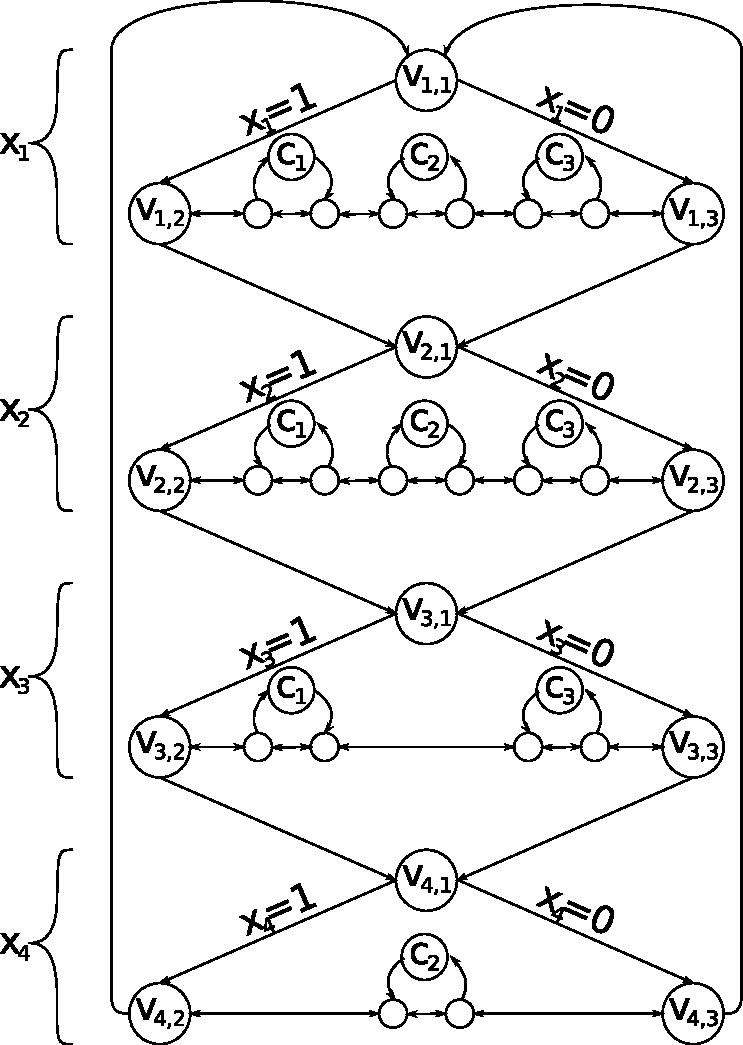
\includegraphics[height=.4\textheight]{kap6BspRed3SatDHC}
      \caption{Die Knoten $v_{i,1}, v_{i,2}, v_{i,3}$, sowie die paarweisen Zwischenknoten zwischen $v_{i,2}$ und $v_{i,3}$ repräsentieren die Variable $x_i$. Von den paarweisen Zwischenknoten geht je eine gerichtete Kante zu einer der Klauseln, die $x_i$ oder $\overline{x}_i$ enthalten. Geht die Kante vom linken Zwischenknoten aus und zum rechten Zwischenknoten zurück, so ist $x_i$ in der Klausel nichtnegiert enthalten. Geht die Kante vom rechten Zwischenknoten aus und zum linken Zwischenknoten zurück, so ist $x_i$ in der Klausel negiert enthalten.}
      \label{kap6BspRed3SatDHC}
    \end{figure}
  \end{Bsp}
  
  Betrachten wir kurz den im Beispiel erstellten Graphen (Abbildung \vref{kap6BspRed3SatDHC}). Wenn wir die Klauselknoten einmal ignorieren, so gibt es genau $2^n$ viele gerichtete Hamiltonkreise, die bei $v_{1,1}$ starten. Das codiert die $2^n$ Belegungen $(v_{i,1} \rightarrow v_{i,2} \rightarrow \ldots \rightarrow v_{i,3} \rightarrow v_{i+1,1} \text{ codiert } x_i = 1 \text{ und } v_{i,1} \rightarrow v_{i,3} \rightarrow \ldots \rightarrow v_{i,2} \rightarrow v_{i+1,1} \text{ codiert } x_i=0)$.
  
  Es sollte klar geworden sein, wie wir die Reduktion vornehmen wollen. Es bleibt zu zeigen, dass $w \in \mathsc{3Sat}$ gilt genau dann, wenn $f(w) \in \mathsc{DHC}$.

  \glq$\Rightarrow$\grq: Es existiere eine erfüllende Belegung $a$. Wähle für $a_i = 1$ die Knoten $v_{i,1} \rightarrow v_{i,2} \rightarrow \ldots$ für $a_i =0$ analog den anderen Pfad. Für jede Klausel $C_j$ gibt es ein erfüllendes Literal ($x_i = 1$ oder $\overline{x}_i = 1$). An den zugehörigen Paaren für $x_i$ (oder $\overline{x}_i$) können wir einen "`Abstecher"' zu $c_j$ machen. Das heißt es existiert ein gerichteter Hamiltonkreis.

  \glq$\Leftarrow$\grq: Es existiere ein gerichteter Hamiltonkreis. Jeder Klauselknoten $c_j$ ist in diesem Kreis enthalten und hat einen Vorgängerknoten $s$ und einen Nachfolgerknoten $t$. Zu zeigen ist, dass $(s,t)$ ist ein Paar sein müssen.
  
  \begin{figure}[htb]
    \centering
    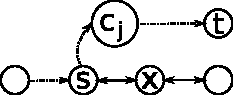
\includegraphics{kap6Red3SatDHCBew1}
    \caption{$s$ und $x$ sind ein Paar im Graphen, wie er in Abbildung \vref{kap6BspRed3SatDHC} dargestellt ist. Die gepunkteten Pfade zeigen den möglichen Verlauf eines Hamiltonkreises, wenn wir davon ausgehen, dass Vorgänger und Nachfolger von $c_j$ kein Paar sein müssen. Die beiden unbezeichneten Knoten gehören entweder zu einem Paar vor beziehungsweise nach $(s,t)$ oder sind die Knoten $v_{i,2}$ beziehungsweise $v_{i,3}$.}
    \label{kap6Red3SatDHCBew1}
  \end{figure}
  
  Angenommen, ein Knoten $c_j$ hätte einen Vorgänger- und einen Nachfolger, die kein Paar sind. Abbildung \vref{kap6Red3SatDHCBew1} zeigt einen möglichen Verlauf eines solchen Hamiltonkreises. Wir verlassen $s$ und gehen zu $c_j$. Wenn wir jetzt nicht zu Knoten $x$ gehen, der ein Paar mit $s$ bildet, so können wir diesen Knoten auf dem Hamiltonkreis nie erreichen. Wir können in einem Hamiltonkreis keinen Knoten zweimal besuchen, $x$ hat jedoch nur zwei Pfade, von denen wir einen bereits besucht haben. Das heißt aus $x$ würde kein Weg mehr herausführen, der nicht gegen die Eigenschaften eines Hamiltonkreises verstoßen würde.

  \begin{figure}[htb]
    \centering
    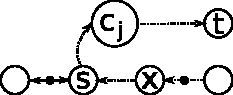
\includegraphics{kap6Red3SatDHCBew2}
    \caption{Auch hier sind $s$ und $x$ ein Paar. Die gepunkteten Pfade zeigen wieder den möglichen Verlauf eines Hamiltonkreises, unter der Annahme, dass Vorgänger und Nachfolger eines Knotens $c_j$ kein Paar sein müssen. Im Unterschied zu Abbildung \vref{kap6Red3SatDHCBew1} haben wir den Knoten $x$ bereits besucht. Wir haben schwarze Zwischenknoten eingefügt vor und nach dem Paar, um zu verdeutlichen, warum die Annahme nicht eintreten kann.}
    \label{kap6Red3SatDHCBew2}
  \end{figure}

  Angenommen wir hätten $x$ vor $s$ besucht. Auch in diesem Fall könnten wir die Eigenschaft des Hamiltonkreises nicht aufrecht erhalten. Um das zu zeigen fügen wir vor den Paaren, nach den Paaren und zwischen den Paaren je einen Zwischenknoten ein. Das ändert die Eigenschaften der gesamten Konstruktion nicht verdeutlicht jedoch das Problem. Abbildung \vref{kap6Red3SatDHCBew2} zeigt, dass wir in einem solchen Fall die gleichen Probleme mit den Zwischenknoten hätten, die bereits zuvor beim Knoten $x$ eingetreten wären (der Zwischenknoten hätte nur zwei Nachbarn, von denen einer bereits besucht wurde).
  
  Es gibt also keinen Hamiltonkreis in dem oben konstruierten Graphen, bei dem der Vorgänger- und Nachfolgerknoten eines Knotens $c_j$ nicht ein Paar sind.
  
  Damit können wir den Hamiltonkreis als Kreis auf den Variablenknoten sehen, in dem an geeigneten Paaren "`Abstecher"' zu den Klauselknoten eingefügt worden sind. In jeder Klausel muss ein Literal $x_i$ erfüllt sein, wenn die Formel erfüllt sein soll. Dies erzwingt eine bestimmte Belegung für $x_i$. Angenommen das Literal ist positiv ($x_i$), so geht vom linken Knoten eines Paares ein gerichteter Weg zum entsprechendem Klauselknoten. Andernfalls ($\overline{x}_i$) geht vom rechten Knoten ein gerichteter Weg zum Klauselknoten und von dort in den linken Knoten des Paares zurück. Ein positives Literal erzwingt also eine Traversierung von links, woraus in unserer Konstruktion $x_i=1$ folgt. Ein negatives Literal erzwingt eine Traversierung von rechts, woraus in unserer Konstruktion $x_i=0$ folgt. Es folgt also $w \in \mathsc{3Sat}$ genau dann, wenn $f(w) \in \mathsc{DHC}$.
\end{Bew}



% Vorlesung 27, 07. Februar 2011 (Mo) Romain Grunert
\section{Weitere Komplexitätsklassen}
\subsection{co-NP}
\begin{Def}[\textsf{co-NP}]
  \hspace{\parindent}\textsf{co-NP} ist die Menge aller Sprachen, deren Komplement in \textsf{NP} ist.
  \[ \operatorname{\mathsf{co-NP}} = \{ L | L^c \in \mathsf{NP} \} \]
\end{Def}

\begin{Bem}
  \hspace{\parindent}$L \in \operatorname{\mathsf{co-NP}}$ heißt man kann in polynomieller Zeit verifizieren, ob $w \notin L$ gilt. Es existiert also ein Polynomialzeitalgorithmus $A$ und ein $k \in \mathbb{N}$, so dass $L=\{ w \mid \forall x \text{ mit } |x| \le |w|^k \text{ gilt } A(w,x)=0 \}$.
\end{Bem}

\begin{Bsp}[Clique\textsuperscript{c}]
  \hspace{\parindent}Betrachten wir kurz ein Beispiel für einen Algorithmus, der sicher in \textsf{co-NP} liegt. Gegeben ist ein Graph $G=(V,E)$ und eine Zahl $g \in \mathbb{N}$. Frage: enthält $G$ keine Clique der Größe $g$?
\end{Bsp}

Man kann leicht verifizieren, ob eine Eingabe nicht zu \textsc{Clique}\textsuperscript{c} gehört. Aber: Wie soll man prüfen beziehungsweise verifizieren, ob eine Eingabe $(G,g)$ zu \textsc{Clique}\textsuperscript{c} gehört? Es ist unbekannt, ob das effizient geht. Die natürlich folgende Frage ist, ob $\mathsf{NP} = \operatorname{\mathsf{co-NP}}$ oder $\mathsf{NP} \neq \operatorname{\mathsf{co-NP}}$? Eine andere interessante Frage ist, ob \textsf{P} eine echte Teilmenge des Schnittes von \textsf{NP} und \textsf{co-NP} ist: $\mathsf{P} \subsetneqq \mathsf{NP} \cap \operatorname{\mathsf{co-NP}}$? Beide Fragen sind bislang unbeantwortet.

\subsection{Jenseits von NP}
Wir wollen weitere Komplexitätsklassen beschreiben. Dazu definieren wir die beiden folgenden Funktionen, wobei $T, S : \mathbb{N} \to \mathbb{N}$:
\begin{itemize}
  \item \textsf{TIME}$(T(n)) :=$ Menge aller Sprachen, die in Zeit $T(n)$ entscheidbar sind.
  \item \textsf{SPACE}$(S(n)) :=$ Menge aller Sprachen, die in Platz $S(n)$ entscheidbar sind.
\end{itemize}


\textsf{P} haben wir bereits wie folgt definiert:
\[ \mathsf{P} = \bigcup_{p \text{ Polynom}} \mathsc{Time}(p(n)) \]

\begin{Def}[\textsf{PSPACE}]
  \hspace{\parindent}Die Komplexitätsklasse \textsf{PSPACE} ist die Menge aller Sprachen, die in polynomiellem Platz entschieden werden können.
  \[ \mathsc{PSpace} := \bigcup_{p \text{ Polynom}} \mathsf{SPACE}(p(n)) \]
\end{Def}

\begin{Bem}
  \hspace{\parindent}Es gilt $\mathsf{TIME}(T(n)) \subseteq \mathsf{SPACE}(T(n))$, also $\mathsf{P} \subseteq \mathsf{PSPACE}$. Eine nichtdeterministische Turingmaschine kann von einer deterministischen Turingmaschine in quadratischem Platz simuliert werden. Also gilt $\mathsf{PSPACE} = \mathsf{NPSPACE}$ und $\mathsf{NP} \subseteq \mathsf{PSPACE}$ und $\operatorname{\mathsf{co-NP}} \subseteq \mathsf{PSPACE}$ (Teil der Übungsaufgaben).
\end{Bem}

\subsubsection{Quantifizierte Boolesche Formeln}
Betrachten wir ein typisches Problem, das in \textsf{PSPACE} liegt: Quantifizierte Boolesche Formeln (\textsc{QBF}). Gegeben ist eine quantifizierte boolesche Formel $\varphi$, das heißt eine Formel der Form
\[ Q_1 x_1 Q_2 x_2 \ldots Q_n x_n \varphi (x_1 \ldots x_n) \]
mit $Q_i \in \{\exists, \forall\}$. Die Grundmenge über die quantifiziert wird ist $x_i \in \{0, 1\}$. Frage: ist $\varphi$ wahr?

\begin{Bsp}
  \hspace{\parindent}Betrachten wir schnell zwei Beispiele:
  \begin{align*}
    \forall x_1 \exists x_2 \forall x_3 (x_1 \vee x_2) \wedge x_3 & \quad\text{ist falsch}\\
    \forall x_1 \exists x_2 \exists x_3 (x_1 \vee x_2) \wedge x_3 & \quad\text{ist wahr}
  \end{align*}
\end{Bsp}

\begin{Satz}
  \hspace{\parindent}$\mathsc{QBF} \in \mathsf{PSPACE}$
\end{Satz}

\begin{Bew}
  \hspace{\parindent}Wir wollen den Beweis nicht komplett durchführen, aber zumindest die Beweisidee darlegen. Man kann eine quantifizierte boolesche Formel, wie folgt umformen:
  \begin{multline*}
    \forall x_1 Q_2 x_2 \ldots Q_n x_n \varphi (x_1 \ldots x_n) \\
    \Leftrightarrow Q_2 x_2 \ldots Q_n x_n \varphi(1, x_2 \ldots x_n) \\ \wedge Q_2 x_2 \ldots Q_n x_n \varphi(0, x_2, \ldots, x_n)
  \end{multline*}
  \begin{multline*}
    \exists x_1 Q_2 \ldots Q_n x_n \varphi(x_1 \ldots x_n) \\
    \Leftrightarrow Q_2 x_2 \ldots Q_n x_n \varphi (1, x_2 \ldots x_n) \\ \vee Q_2 x_2 \ldots Q_n x_n \varphi(0, x_2 \ldots x_n)
  \end{multline*}
  
  Damit kann man rekursiv bestimmen, ob $Q_1 x_1 \ldots Q_n x_n \varphi(x_1 \ldots x_n)$ wahr ist. Beim zweiten rekursiven Aufruf kann man den Platz des ersten Aufrufs wiederverwenden. Dadurch bleibt der Platzbedarf polynomiell. Das zu zeigen geht jedoch über die Beweisidee hinaus.
\end{Bew}

Noch einfacher ist $\mathsc{Sat} \le_p \mathsc{QBF}$ zu zeigen. Eine Eingabe für \textsc{Sat} $\varphi(x_1 \ldots x_n)$ in KNF ist genau dann erfüllbar, wenn $\exists x_1 \ldots \exists x_n \varphi(x_1 \ldots x_n)$ wahr ist. Damit wäre auch gezeigt, dass \textsc{QBF} \textsf{NP}"=schwer ist. Es lässt sich sogar zeigen, dass $L \le_p \mathsc{QBF}$ für alle $L \in \mathsf{PSPACE}$ gilt (hier ohne Beweis). \textsc{QBF} liegt wie oben gezeigt in \textsf{PSPACE} und es lassen sich alle Probleme aus \textsf{PSPACE} darauf poynomiell reduzieren. Daraus folgt, dass \textsc{QBF} \textsf{PSPACE}"=vollständig ist.

\subsubsection{Geo}
Betrachten wir noch ein anderes Problem: \textsc{Geo}, ein verallgemeinertes Geographiespiel. Gegeben ist ein gerichteter Graph $G=(V,E)$. Das Spiel verläuft wie folgt: Spieler $A$ setzt einen Stein auf einen Knoten, Spieler $B$ setzt einen Stein auf einen Nachfolgerknoten, und so weiter. Als Regel (oder Nebenbedingung) definieren wir, dass auf jeden Knoten nur ein Stein gesetzt werden darf. Es ergibt sich also ein Pfad. Verloren hat derjenige Spieler, der nicht mehr regelkonform setzen kann.

Das Problem besteht aus der Frage, ob der Spieler, der anfängt eine Gewinnstrategie haben kann? Das heißt: existiert ein Zug für Spieler $A$, so dass für alle Züge von Spieler $B$ gilt, dass er einen Gewinn von $A$ nicht mehr abwenden kann?

Es gilt $\mathsc{QBF} \le_p \mathsc{Geo}$. Daraus folgt, dass \textsc{Geo} \textsf{PSPACE}"=vollständig ist (hier ohne Beweis).

Es gilt $\mathsf{NP} \subseteq \mathsf{PSPACE}$ und demnach auch $\mathsf{P} \subseteq \mathsf{PSPACE}$. Es ist bislang nicht geklärt ob auch $\mathsf{NP} \subsetneqq \mathsf{PSPACE}$ und/oder $\mathsf{P} \subsetneqq \mathsf{PSPACE}$ gelten.

\subsection{Jenseits von PSPACE}
\begin{Def}[\textsf{EXPTIME}]
  \hspace{\parindent}Die Komplexitätsklasse \textsf{EXPTIME} ist die Menge aller Sprachen, die in exponentieller Zeit entschieden werden können.
  \[ \mathsf{EXPTIME} = \bigcup_{\substack{\text{Konstante c} \\ \text{Polynom p}}} \mathsf{TIME}(c^{p(n)}) \]
\end{Def}

Im Folgenden wollen wir zeigen, dass $\mathsf{PSPACE} \subseteq \textsf{EXPTIME}$ und $\mathsf{P} \subsetneqq \textsf{EXPTIME}$ gelten.

\begin{Satz}
  \hspace{\parindent}Ist ein Problem lösbar mit $S(n)$ Platz, so auch in $c^{S(n)}$ Zeit für eine Konstante $c$.
\end{Satz}

\begin{Bew}
  \hspace{\parindent}Den vollständigen Beweis gehen wir hier nicht durch, jedoch die Beweisidee sollte klar werden. Eine Turingmaschine $M$ verbraucht auf einem Band $S(n)$ Platz unter Nutzung eines Alphabetes der Größe $a$, also $|\Sigma|=a$. Eine Turingmaschine verfügt über eine endliche Kontrolle, $M$ habe $b$ viele Zustände. Daraus folgt, es sind maximal $S(n)$ verschiedene Kopfpositionen möglich und maximal $a^{S(n)}$ viele verschiedene Bandinhalte. Insgesamt gibt es also höchstens $S(n) \cdot a^{S(n)} \cdot b$ mögliche Konfigurationen. Da sich keine Konfiguration wiederholen darf (sonst gerät $M$ in eine Endlosschleife), muss die Laufzeit $\le c^{S(n)}$ sein, für eine geeignete Konstante $c$. Es folgt
  \[ \mathsf{SPACE}(S(n)) \subseteq \bigcup_{c \ge 1} \mathsf{TIME}(c^{S(n)}) \]
  und daher 
  \[ \mathsf{PSPACE} \subseteq \mathsf{EXPTIME} \]
  Offen ist, ob $\mathsf{PSPACE} \subsetneqq \mathsf{EXPTIME}$ und/oder $\mathsf{NP} \subsetneqq \mathsf{EXPTIME}$ gelten.
\end{Bew}

Man möchte die verschiedenen Komplexitätsklassen so gut, wie möglich von einander abgrenzen. Statt von $\subseteq$ sprechen zu müssen, möchte man, wo möglich, den Nachweis führen, dass eine Komplexitätsklasse eine echte Teilmenge einer anderen Komplexitätsklasse ist. Es gibt dabei zwei Einschränkungen: die Klassen müssen das gleiche Berechnungsschema zu Grunde legen (zum Beispiel eine TM) und die gleiche Ressource (Raum oder Zeit) betrachten. Solche Beweise nennt man Hierarchiesätze, weil sie die Klassen der betrachteten Ressource (\textsf{TIME}, \textsf{SPACE}) hierarchisch ordnen. Wir wollen folgende Hierarchiesätze angeben, ohne die zugehörigen Beweise näher zu betrachten. Für "`hinreichend vernünftige"' Funktionen gilt:
\begin{enumerate}
  \item Ist $S_1 = o(S_2)$, so ist $\mathsf{SPACE}(S_1) \subsetneqq \mathsf{SPACE}(S_2)$
  \item Ist $T_1 \log T_1 = o(T_2)$, so ist $\mathsf{TIME}(T_1) \subsetneqq \mathsf{TIME}(T_2)$.
\end{enumerate}

Mit Hilfe des zweiten Satzes (der auch \textit{Zeithierarchiesatz} genannt wird) können wir leicht zeigen, dass $\mathsf{P} \subsetneqq \textsf{EXPTIME}$ gilt:

\begin{Bew}
  \hspace{\parindent}Sei $p(n)$ ein Polynom. Dann gilt: $p(n) \log p(n) = o(2^{\nicefrac{n}{2}})$. Das heißt 
  \[ \lim_{n \to \infty} \frac{p(n) \log p(n)}{2^{\nicefrac{n}{2}}} = 0 \]
  Daraus folgt $\mathsf{P} \subseteq \mathsf{TIME}(2^{\nicefrac{n}{2}})$. Da $2^{\nicefrac{n}{2}} \log 2^{\nicefrac{n}{2}} = 2^{\nicefrac{n}{2}} \cdot \frac{n}{2} = o(2^n)$ gilt nach dem Zeithierarchiesatz $\mathsf{TIME}(2^{\nicefrac{n}{2}}) \subsetneqq \mathsf{TIME}(2^n)$.
  
  Daher gilt
  \[ \mathsf{P} \subseteq \mathsf{TIME}(2^{\nicefrac{n}{2}}) \subsetneqq \mathsf{TIME}(2^n) \subseteq \mathsf{EXPTIME} \]
  also
  \[ \mathsf{P} \subsetneqq \mathsf{EXPTIME} \]
\end{Bew}

Wir wissen $\mathsf{P} \subseteq \mathsf{NP} \subseteq \mathsf{PSPACE} \subseteq \mathsf{EXPTIME}$ und $\mathsf{P} \subsetneqq \mathsf{EXPTIME}$. Mindestens eine der Teilmengen muss also echt sein, es ist bislang jedoch noch nicht bekannt welche. Es ist also unklar ob $\mathsf{P} \subsetneqq \mathsf{NP}$, $\mathsf{NP} \subsetneqq \mathsf{PSPACE}$ und/oder $\mathsf{PSPACE} \subsetneqq  \mathsf{EXPTIME}$ gilt und dann dem entsprechend $\mathsf{P} \neq \mathsf{NP}$, $\mathsf{NP} \neq  \mathsf{PSPACE}$ und/oder $\mathsf{PSPACE} \neq  \mathsf{EXPTIME}$ gilt.

\subsection{Nachweisbar schwere Probleme}
Alle bisher vorgestellten Probleme können auch in \textsf{P} liegen. Es gibt jedoch auch Probleme, von denen bewiesen ist, dass sie nicht in \textsf{P} sind. Wir betrachten beispielhaft Äquivalente reguläre Ausdrücke (\textsc{ÄRA}).

Gegeben sind zwei reguläre Ausdrücke $e_1$ und $e_2$ mit $\cup, \cdot, *, \overline{~}, \cap$, zum Beispiel $aa* \cup \varepsilon$ und $\overline{a* b a* \cup b* a b*}* \cap a*$. Beschreiben $e_1$ und $e_2$ die gleiche Sprache $L(e_1) = L(e_2)$?

\begin{Satz}
  \hspace{\parindent}$\textsc{ÄRA} \in \mathsf{EXPTIME}$
\end{Satz}

\begin{Bew}
  \hspace{\parindent}Ein Regulärer Ausdruck lässt sich polynomiell in einen NFA (nichtdeterministischen endlichen Automaten) überführen, der lässt sich exponentiell in einen DFA (endlichen deterministischen Automaten) überführen, der lässt sich polynomiell in einen minimalen DFA überführen. Da es zu jedem DFA einen (bis auf die Benennung der Zustände) eindeutigen minimalen DFA gibt, lässt sich somit überprüfen, ob die beiden regulären Ausdrücke die selbe Sprache beschreiben, die der minimale DFA erkennt.
\end{Bew}
\begin{Satz}
  \hspace{\parindent}Jeder Algorithmus, der \textsc{ÄRA} löst, hat Laufzeit $\Omega(c^{\sqrt{\frac{n}{\log n}}})$ für ein $c > 1$ Daraus folgt ÄRA ist nicht in \textsf{P}.
\end{Satz}

Den Satz geben wir hier ohne Beweis an.


\section{Zusammenfassung und Übersicht}
Um uns eine abschließende Übersicht zu verschaffen, wollen wir zusammenfassen. \textsf{NP} ist die Klasse der Probleme, die von eine nichtdeterministischen Turingmaschine in polynomieller Zeit berechnet werden können, beziehungsweise die Klasse der Probleme, deren Lösung von einer deterministischen Turingmaschine in polynomieller Zeit überprüft werden können (das widerspricht sich nicht, siehe oben). \textsf{P} ist die Komplexitätsklasse der Probleme, die von einer deterministischen Turingmaschine in polynomieller Zeit gelöst werden können. $\mathsf{P} \subset \mathsf{NP}$ gilt sicher. Unklar ist, ob sogar $\mathsf{P} = \mathsf{NP}$ gilt oder ob viel mehr $\mathsf{P} \neq \mathsf{NP}$ gilt. Diese Frage wird \textsf{P}-\textsf{NP}-Problem genannt und gilt als eine der wichtigsten Fragen der Informatik. Zumeist wird von $\mathsf{P} \neq \mathsf{NP}$ ausgegangen, dies ist bislang aber unbewiesen.

\begin{figure}[htb]
  \centering
  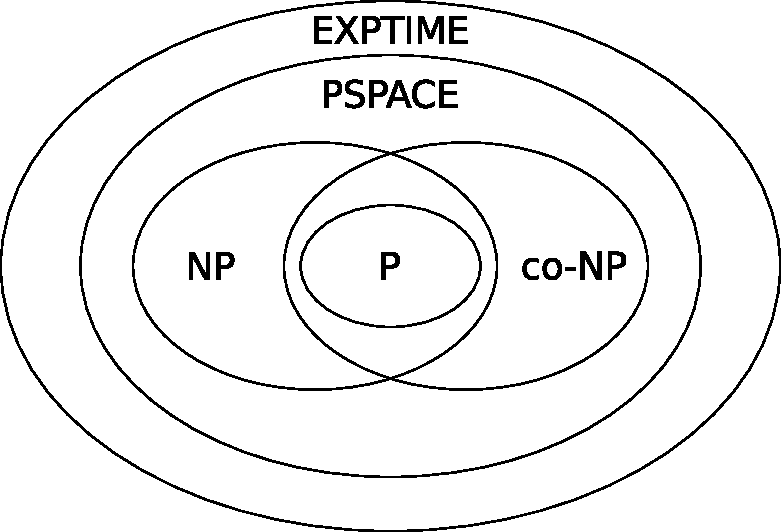
\includegraphics[scale=.6]{kap6Komplexitaetsklassen}
  \caption{Gezeigt wird das Verhältnis der Komplexitätsklassen zueinander, unter der Annahme, dass $\mathsf{P} \neq \mathsf{NP}$, dass $\operatorname{\mathsf{co-NP}} \neq \mathsf{NP}$, dass $\mathsf{P} \subsetneqq \mathsf{NP} \cap \operatorname{\mathsf{co-NP}}$ und $\mathsf{NP} \subsetneqq \mathsf{PSPACE}$.}
  \label{kap6Komplexitaetsklassen}
\end{figure}

\textsf{co-NP} ist die Klasse der Probleme, deren Komplement in \textsf{NP} liegt. Es ist unklar, ob $\operatorname{\mathsf{co-NP}} = \mathsf{NP}$ oder $\operatorname{\mathsf{co-NP}} \neq \mathsf{NP}$. \textsf{PSPACE} ist die Klasse der Sprachen, die unter polynomiellen Platzbedarf gelöst werden können. \textsf{EXPTIME} ist die Klasse der Sprachen, die in exponentieller Zeit gelöst werden können. Abbildung \vref{kap6Komplexitaetsklassen} veranschaulicht das.

Das Mittel der Polynomialzeit"=Reduktion erlaubt es ein Problem zu lösen, in dem die Eingabe in eine Eingabe für ein anderes Problem in polynomieller Zeit gewandelt wird. Dabei kann die gewandelte Eingabe genau dann gelöst werden, wenn es auch für die originale Eingabe möglich ist. Ein Problem heißt \textsf{NP}-schwer, wenn alle Probleme die in \textsf{NP} liegen in polynomieller Zeit auf das Problem reduziert werden können. Liegt das Problem selbst auch in \textsf{NP}, so nennt man es \textsf{NP}"=vollständig. Könnte für ein Problem aus \textsf{P} gezeigt werden, dass es \textsf{NP}-schwer ist, so wäre $\mathsf{P} = \mathsf{NP}$ bewiesen.

\begin{figure}[htb]
  \centering
  \includegraphics[scale=.6]{kap6ReduktionenUebersicht}
  \caption{Wir haben für \textsc{CSat} gezeigt, dass es \textsf{NP}"=vollständig ist. Für die anderen hier gezeigten Probleme haben wir durch Reduktion gezeigt, dass auch sie \textsf{NP}-schwer sind. Alle diese Probleme liegen in \textsf{NP} und sind somit \textsf{NP}"=vollständig.}
  \label{kap6ReduktionenUebersicht}
\end{figure}

Wir haben für eine Reihe von Problemen gezeigt, dass sie \textsf{NP}"=vollständig sind. Angefangen haben wir mit \textsc{CSat}, das wir auf weitere Probleme reduziert haben. Da Reduktion transitiv ist, gilt somit auch für diese Probleme, dass sie \textsf{NP}"=vollständig sind. Hat man ein \textsf{NP}"=vollständiges Problem auf ein andere Problem reduziert, dass auch in \textsf{NP} liegt, so weiß man auch, dass die Reduktion in die andere Richtung möglich ist, ohne es zeigen zu müssen (bedingt sich durch die Definition von \textsf{NP}-schwer). Abbildung \ref{kap6ReduktionenUebersicht} verschafft einen Überblick über die Probleme, für die wir \textsf{NP}"=Vollständigkeit gezeigt haben.
%Wenn \textsc{CSat} \textsf{NP}-Schwer und $\mathsc{Sat} \in \mathsf{NP}$, dann muss die "`Gegenrichtung"' wegen des Satz von Cook nicht mehr gezeigt werden.
